
\section{Simulation Test and Analysis}


This section presents a thorough exploration of the proposed complete coverage path planning algorithm tailored for agricultural field applications. It unfolds into two distinct sections:

\vspace*{6mm}  

\textbf{Simulation Setup:} 

This section is dedicated to providing a detailed exposition of the simulation setup. Meticulous attention is directed towards delineating the experimental framework within which the simulation tests are conducted.

\vspace*{6mm}  

\textbf{Simulation Results and Analysis:}  

Comprehensive empirical findings obtained from the meticulously designed simulation experiments within the aforementioned framework are detailed in this section. Key performance metrics are analyzed to provide a holistic assessment of the algorithm's performance under diverse scenarios. we conduct a thorough analysis of the empirical results, meticulously scrutinizing each detail. Through this examination, we aim to discern the operational dynamics of the algorithm, identify its strengths, and pinpoint areas for potential refinement.
\vspace*{6mm}   

\subsection{Simulation Setup}


The simulation setup is meticulously designed to emulate the real-world operational environment of an agricultural field, ensuring that the algorithm's performance can be rigorously tested under realistic conditions. The global coverage path planning is initially performed using Matplotlib, followed by testing in a simulation environment leveraging the Robot Operating System (ROS) and the Gazebo simulator.

\vspace*{6mm}  

In the context of coverage path planning for agricultural fields, it is crucial to account for varying plant distributions. Therefore, different datasets are used to represent diverse scenarios, with the aim of assessing the algorithm's robustness under varying initial conditions and plant distributions. Specifically, the simulation setup incorporates different datasets with the same initial position and orientation of the robot to demonstrate the algorithm's adaptability.

\vspace*{6mm}  

Dataset Description:


To comprehensively evaluate the algorithm, six distinct datasets are employed within the flat field of 120m x 120m area, with each dataset containing different numbers of points: 250, 500, 2000, 4000, 6000, and 10,000. Each primary dataset is further subdivided into four sub-datasets, characterized by different spatial distributions:

\begin{itemize}
    \item Random Distribution: Points are distributed randomly throughout the field.
    \item Clustered Distribution (4 Clusters): 20\% of the points are distributed randomly, while 80\% are distributed in four clusters with distinct Gaussian distribution variances.
    \item Clustered Distribution (6 Clusters): 20\% of the points are distributed randomly, with the remaining 80\% distributed in six clusters, each with distinct means and variances.
    \item Clustered Distribution (10 Clusters): 20\% of the points are randomly distributed, and 80\% are in ten clusters, each characterized by unique Gaussian distribution parameters.
\end{itemize}

This results in a total of 24 different datasets, meticulously crafted to test the algorithm's robustness across various scenarios, including variations in the number of points, their distribution patterns, the number of clusters, and the statistical properties of these clusters. Such comprehensive testing ensures that the algorithm is robust and adaptable to real-world agricultural environments, where plant distributions can significantly vary.

\vspace*{6mm}  

Performance Metrics
The performance of the algorithm is evaluated using several critical metrics across all datasets:

\begin{itemize}
    \item Computational Time: The time required for the algorithm to compute the coverage path.
    \item Field Operation Time: The actual time taken for the robot to complete the coverage task.
    \item Total Path Length: The total distance traveled by the robot.
    \item Number of Turns: The total number of turns the robot makes during its operation.
    \item Energy Consumption: The energy used by the robot to complete the coverage task.
    \item Coverage Efficiency: The percentage of points covered by the robot within the operational time.
\end{itemize}
These metrics provide a comprehensive assessment of the algorithm's efficiency, effectiveness, and overall performance under different test scenarios.

\vspace*{6mm}  

\textbf{Processor Specifications:}


Processor: AMD® Ryzen 5 Pro 5675U with Radeon Graphics x 12.


Processing Speed: 2.3 GHz, Number of Cores: 6, and RAM: 16 GB.


\vspace*{6mm}  

\textbf{Visual Representation of the Dataset}

The distribution of points across the different datasets can be visualized in (\autoref{fig:Dataset}), illustrating the varying scenarios used to test the algorithm's robustness.


% % % % % Dataset visualization
% % % % \begin{figure}[p]
% % % %     \centering
% % % %     \begin{tabular}{ccc}
% % % %          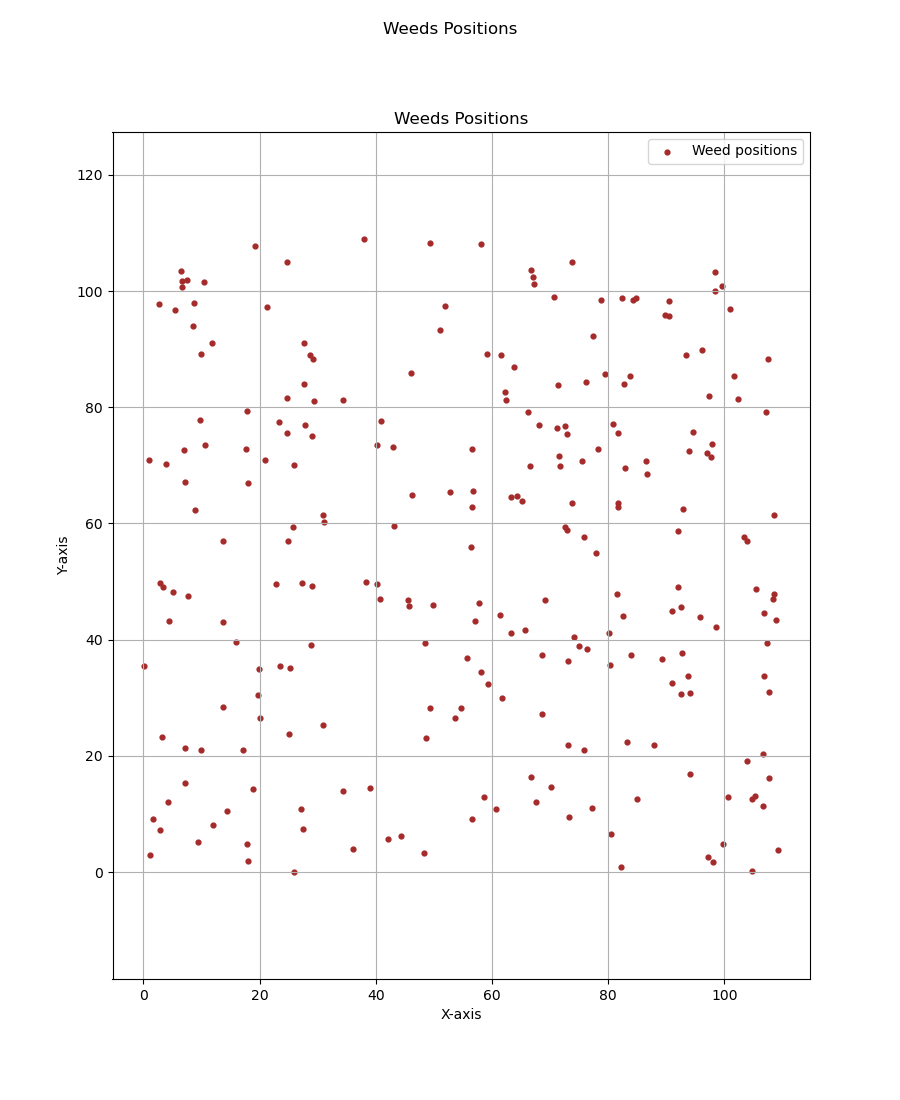
\includegraphics[height=36mm,width=0.24\textwidth]{Images/data/01.png}
% % % %         & 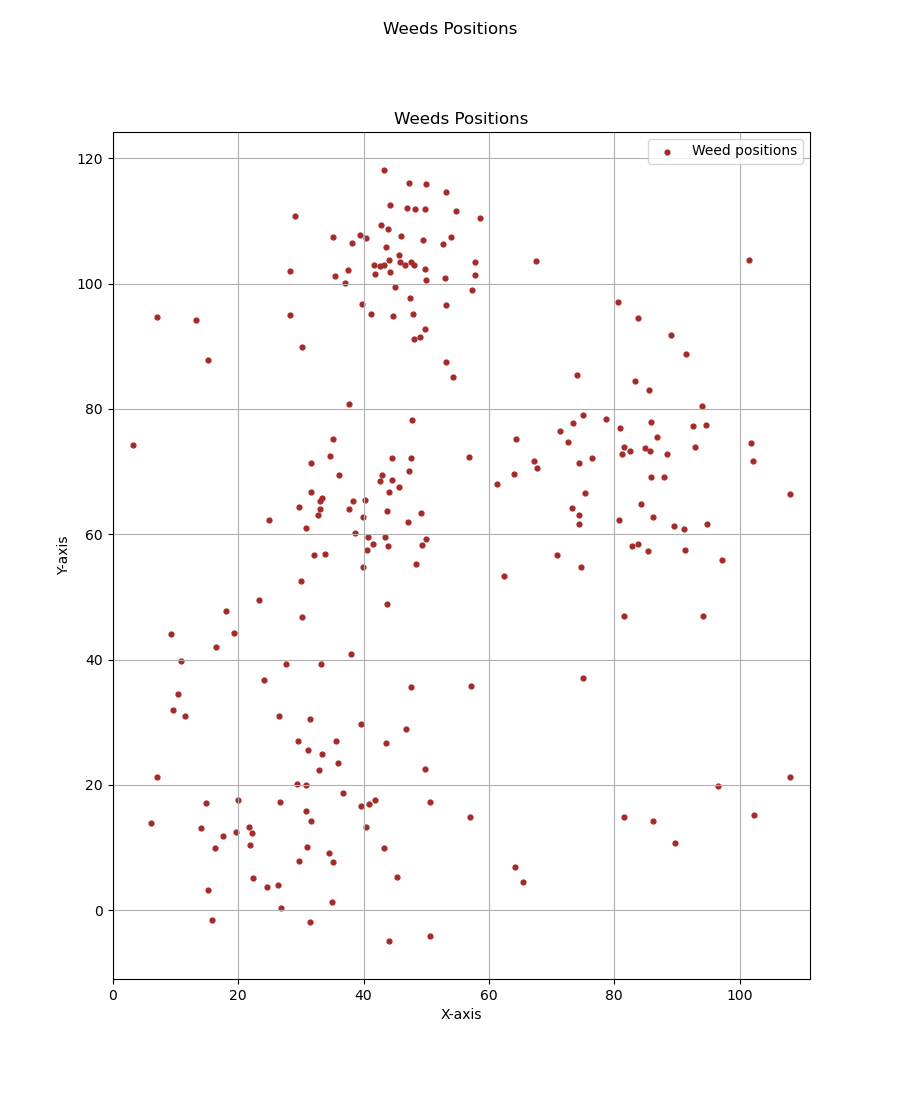
\includegraphics[height=36mm,width=0.24\textwidth]{Images/data/02.png}
% % % %         & 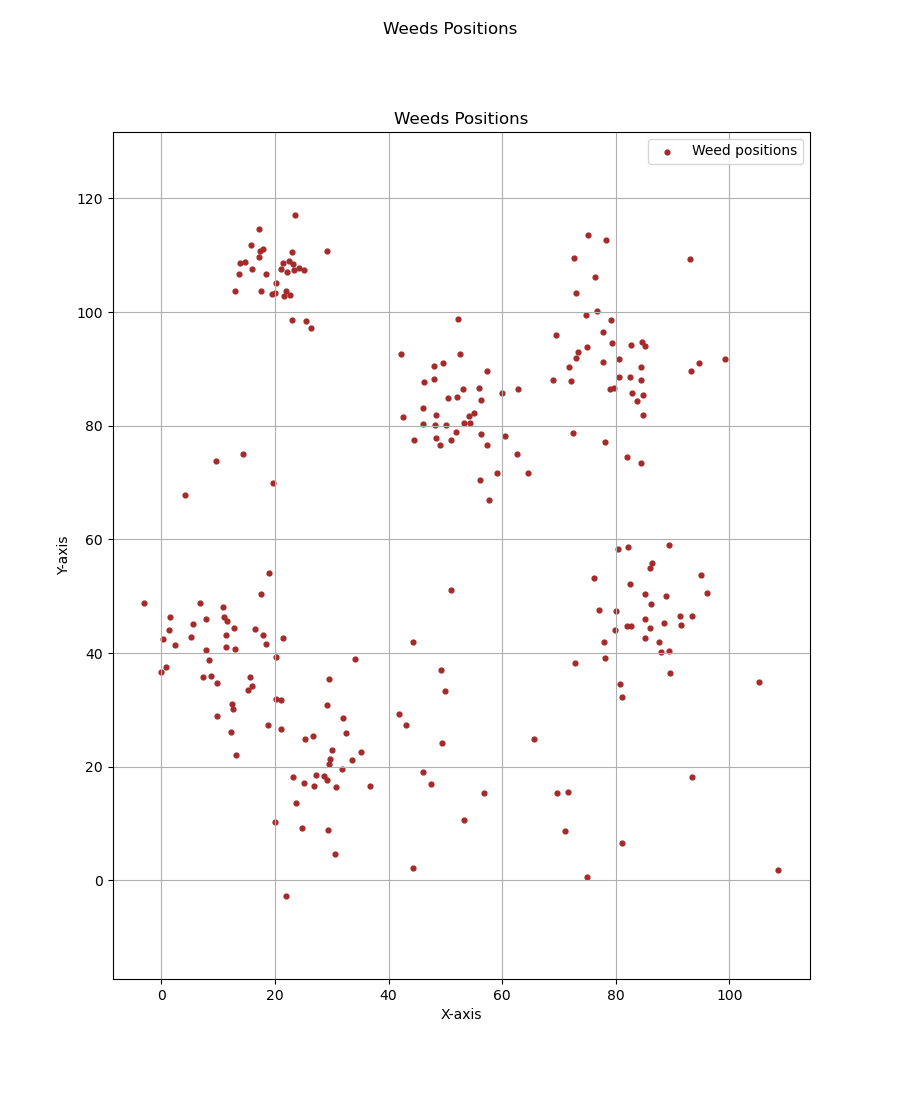
\includegraphics[height=36mm,width=0.24\textwidth]{Images/data/03.png}
% % % %          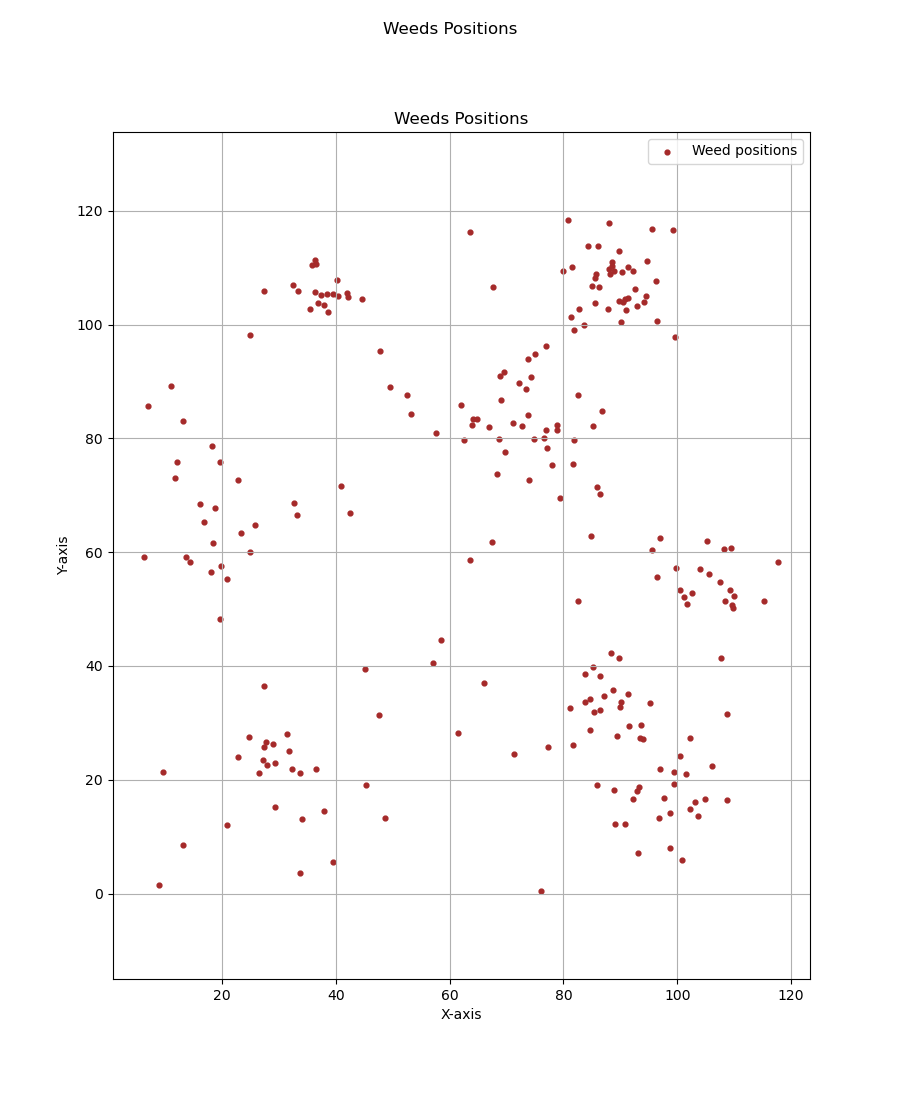
\includegraphics[height=36mm,width=0.24\textwidth]{Images/data/04.png}\\[-4pt]

% % % %         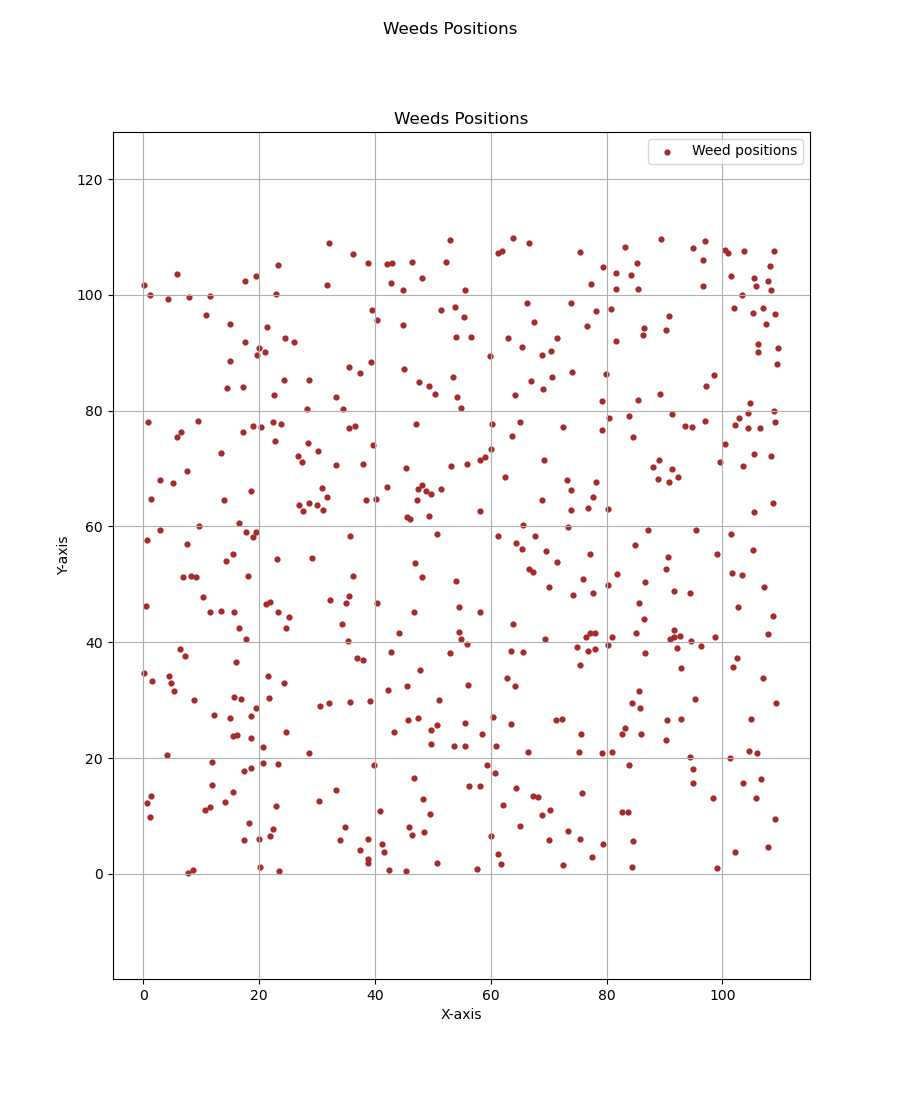
\includegraphics[height=36mm,width=0.24\textwidth]{Images/data/11.png}
% % % %         & 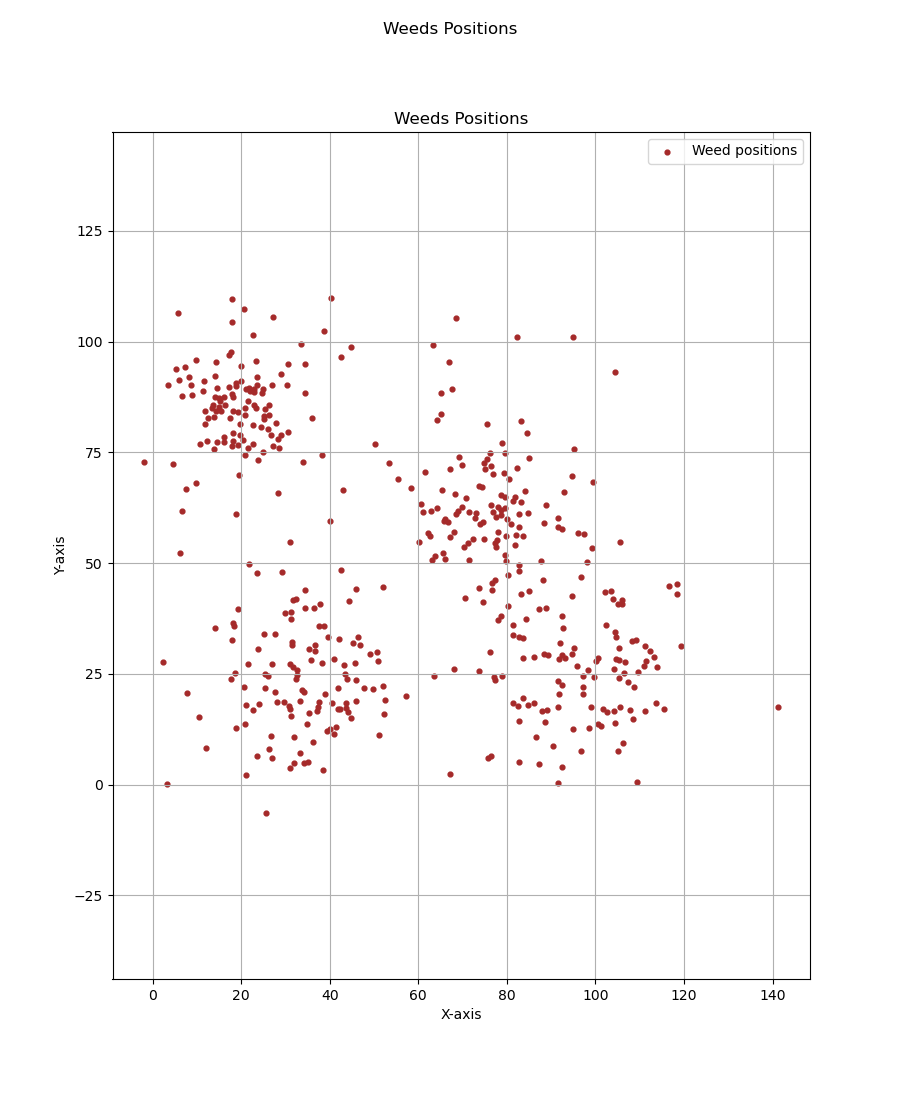
\includegraphics[height=36mm,width=0.24\textwidth]{Images/data/12.png}
% % % %         & 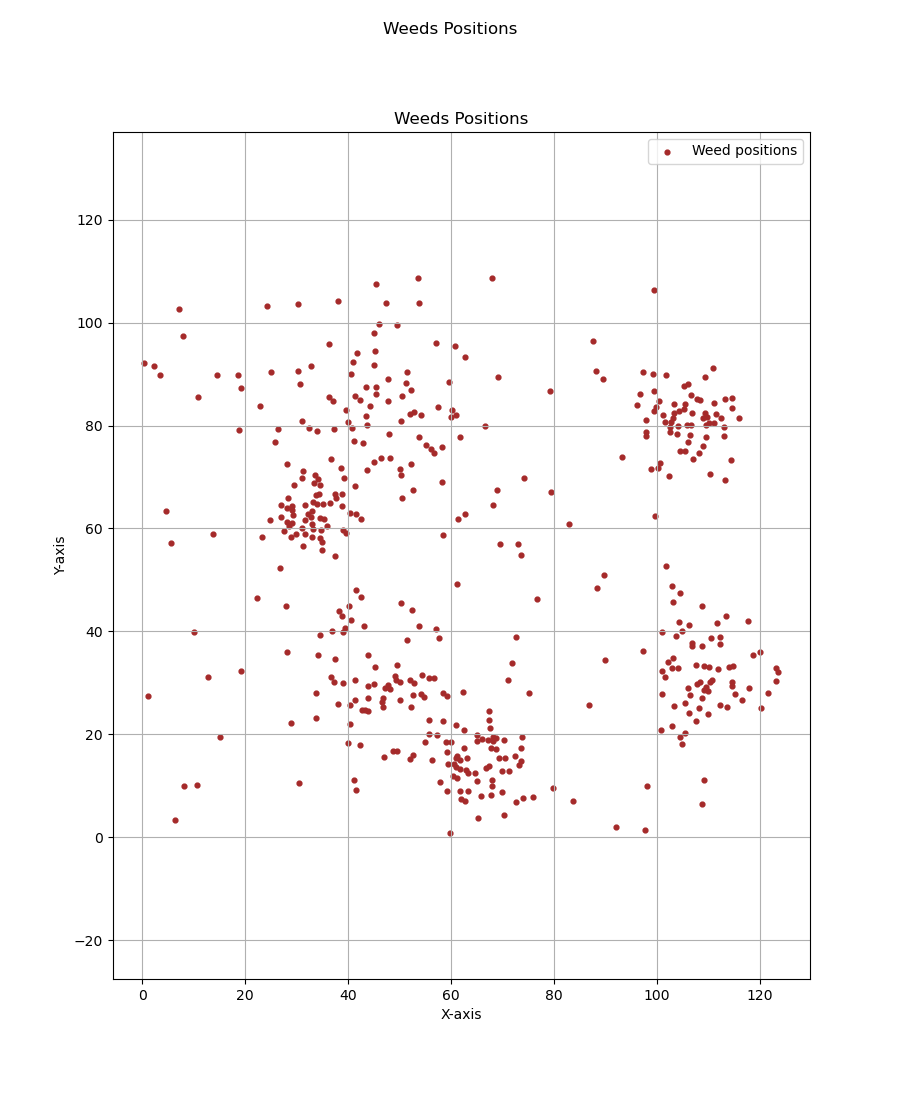
\includegraphics[height=36mm,width=0.24\textwidth]{Images/data/13.png}
% % % %         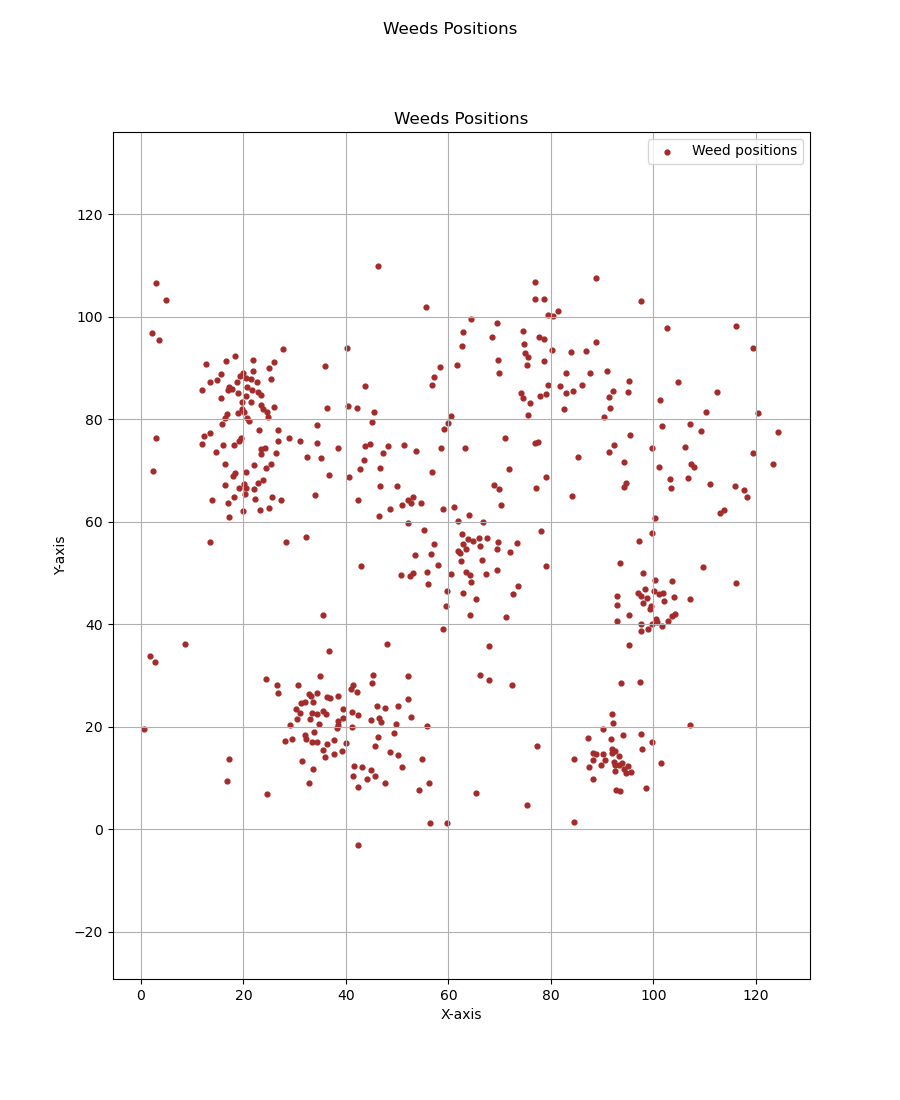
\includegraphics[height=36mm,width=0.24\textwidth]{Images/data/14.png}\\[-4pt]

% % % %         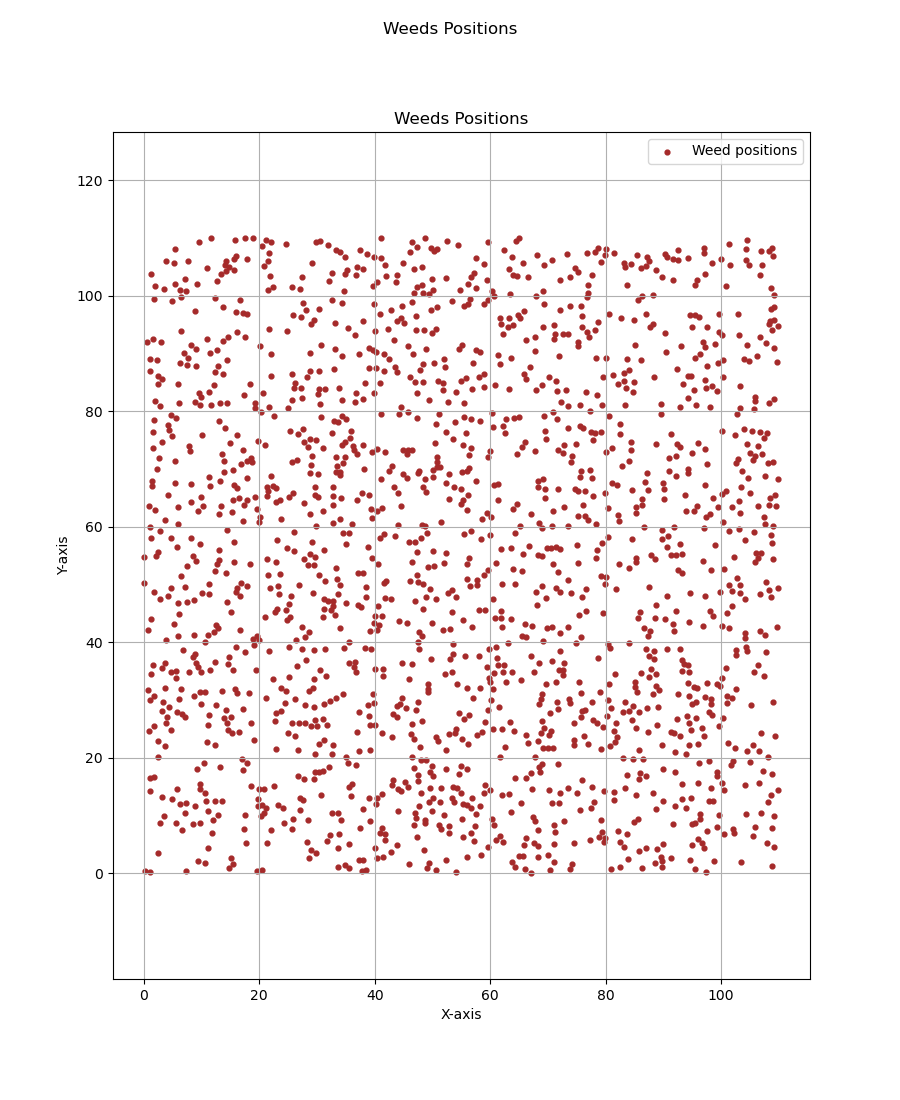
\includegraphics[height=36mm,width=0.24\textwidth]{Images/data/21.png}
% % % %         & 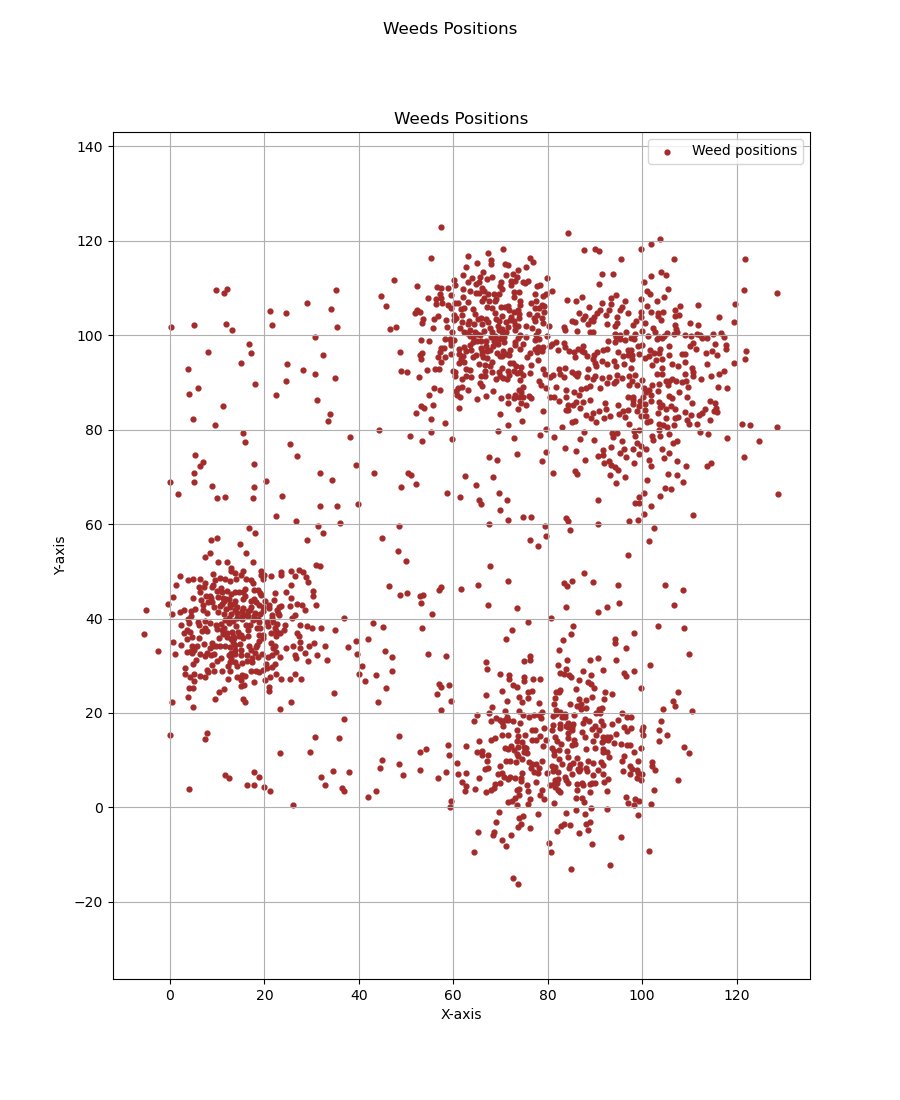
\includegraphics[height=36mm,width=0.24\textwidth]{Images/data/22.png}
% % % %         & 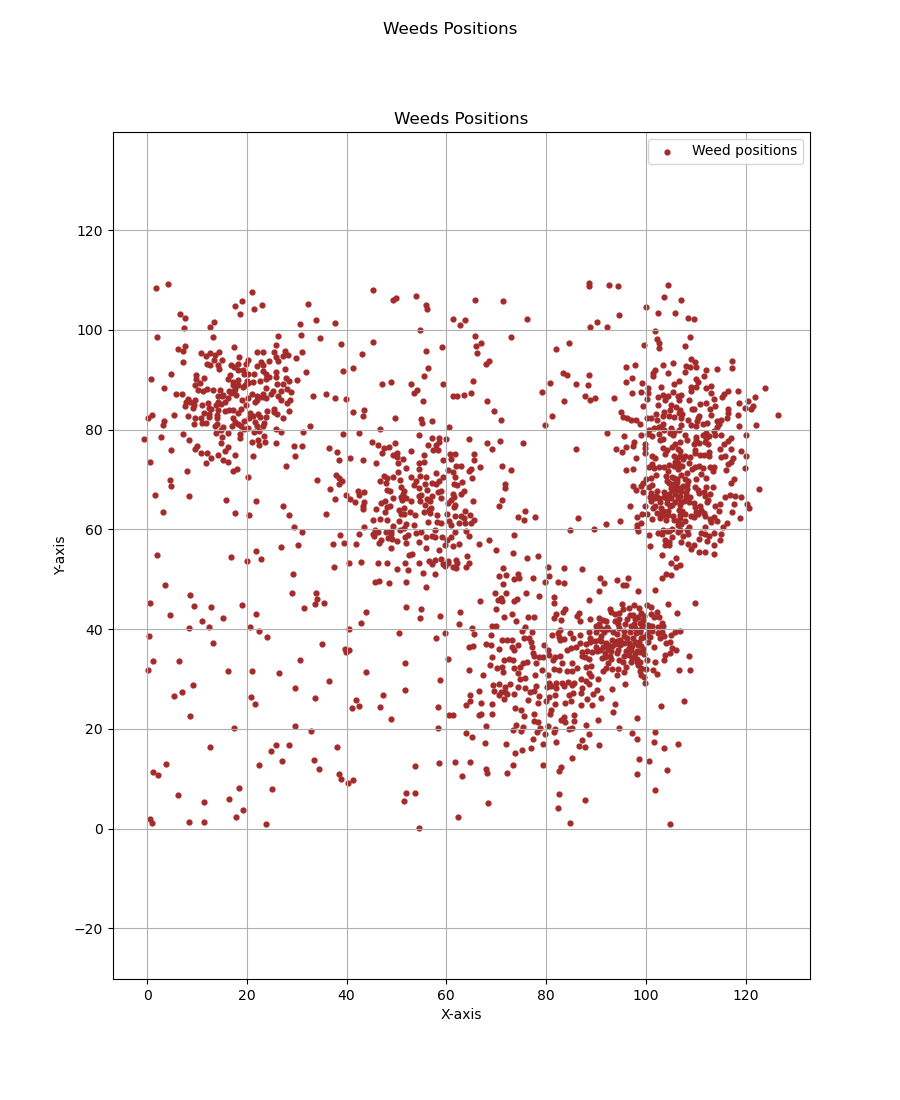
\includegraphics[height=36mm,width=0.24\textwidth]{Images/data/23.png}
% % % %          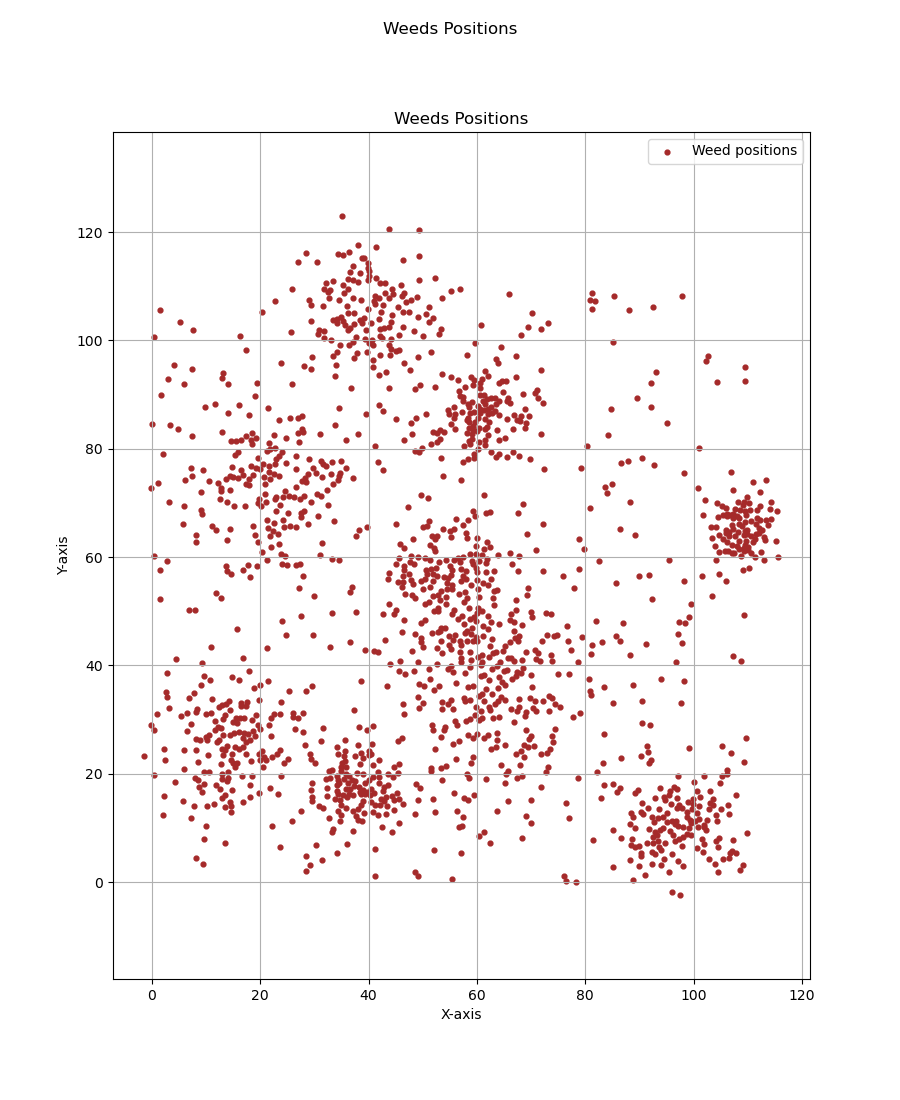
\includegraphics[height=36mm,width=0.24\textwidth]{Images/data/24.png}\\[-4pt]

% % % %          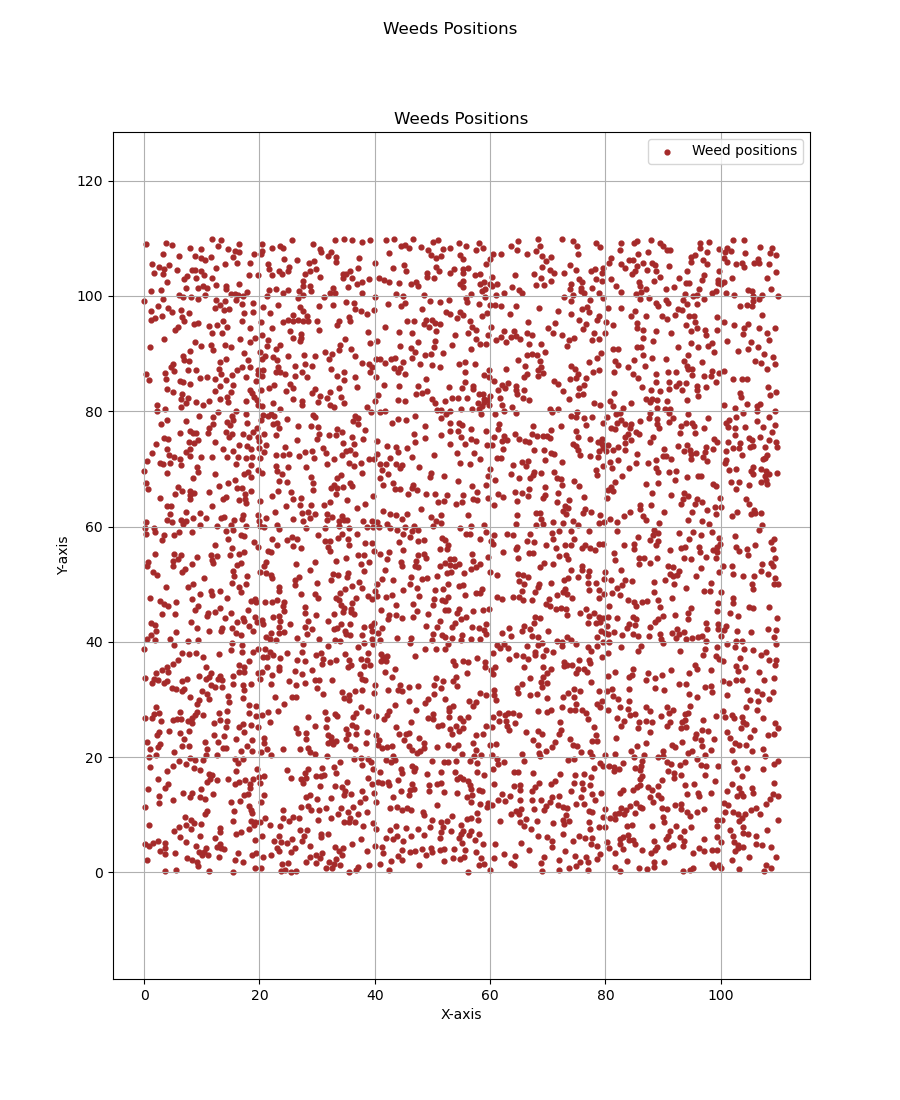
\includegraphics[height=36mm,width=0.24\textwidth]{Images/data/31.png}
% % % %         & 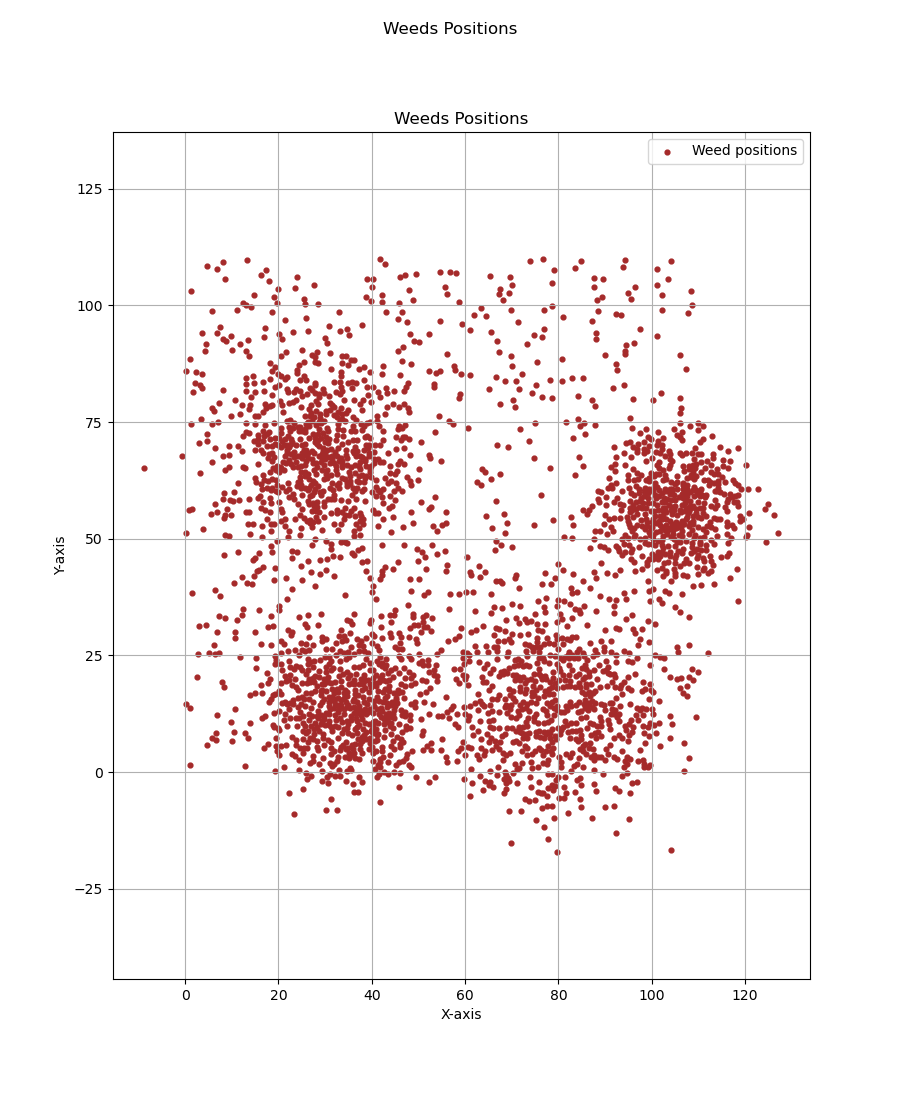
\includegraphics[height=36mm,width=0.24\textwidth]{Images/data/32.png}
% % % %         & 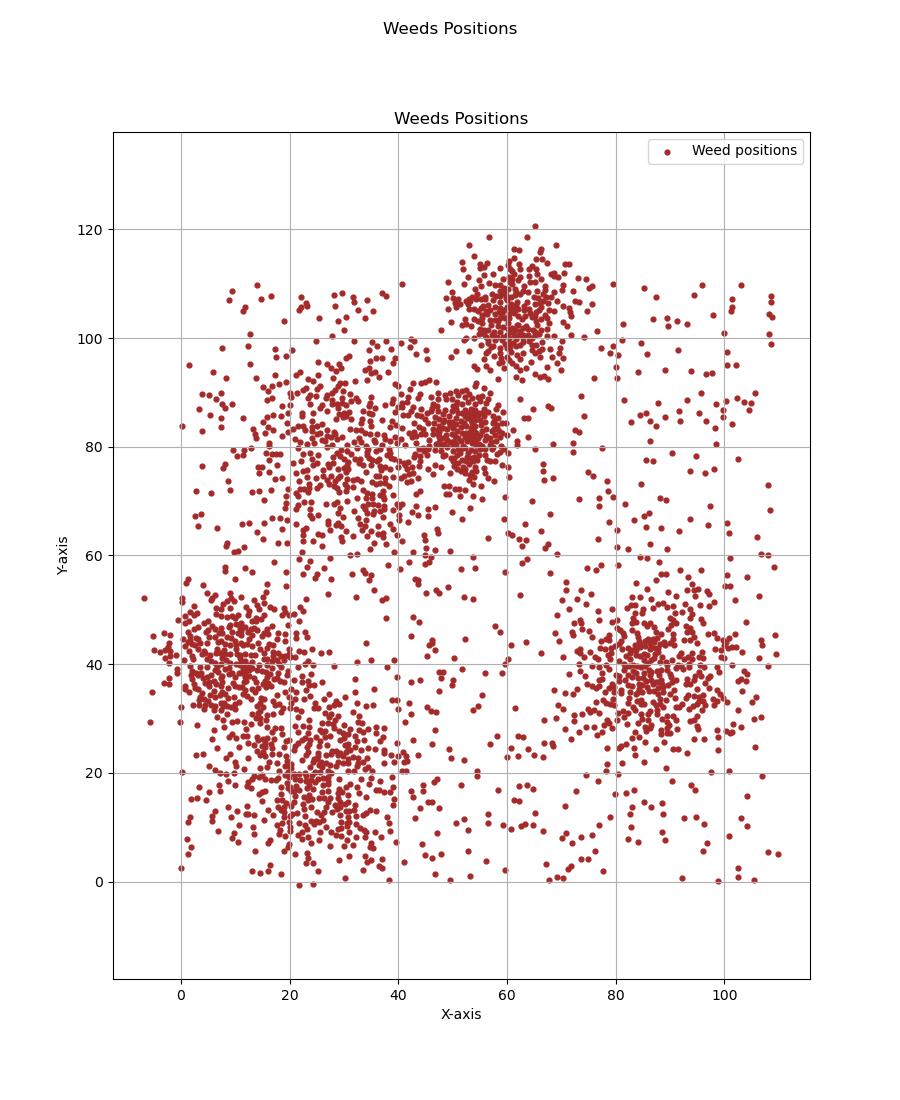
\includegraphics[height=36mm,width=0.24\textwidth]{Images/data/33.png}
% % % %          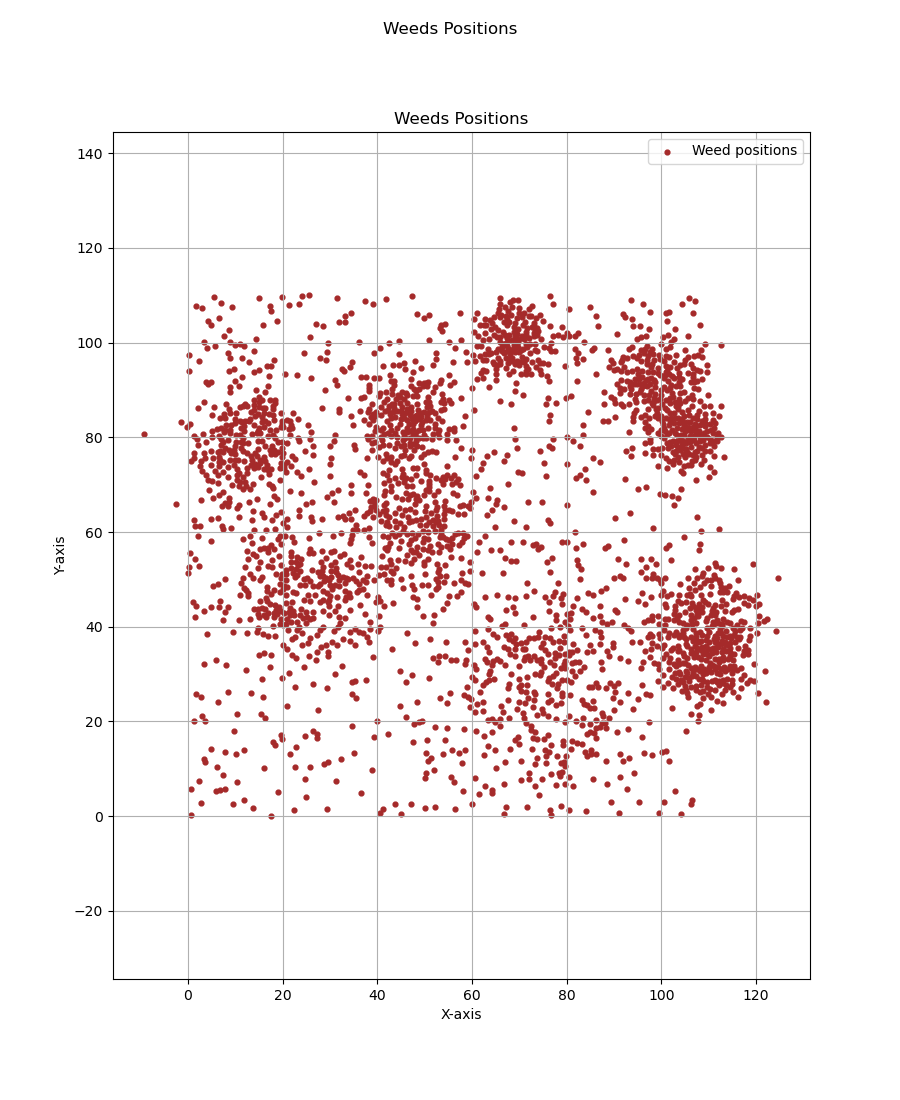
\includegraphics[height=36mm,width=0.24\textwidth]{Images/data/34.png}\\[-4pt]


% % % %         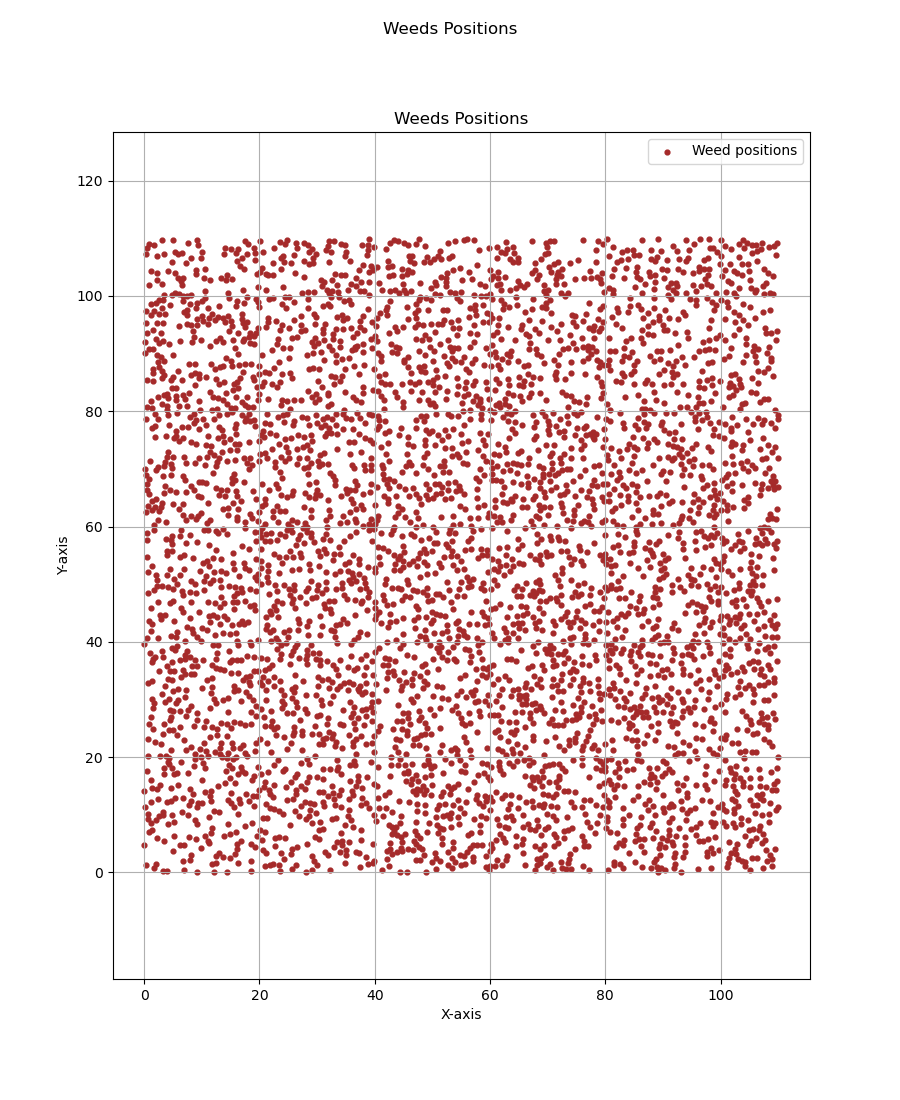
\includegraphics[height=36mm,width=0.24\textwidth]{Images/data/41.png}
% % % %         & 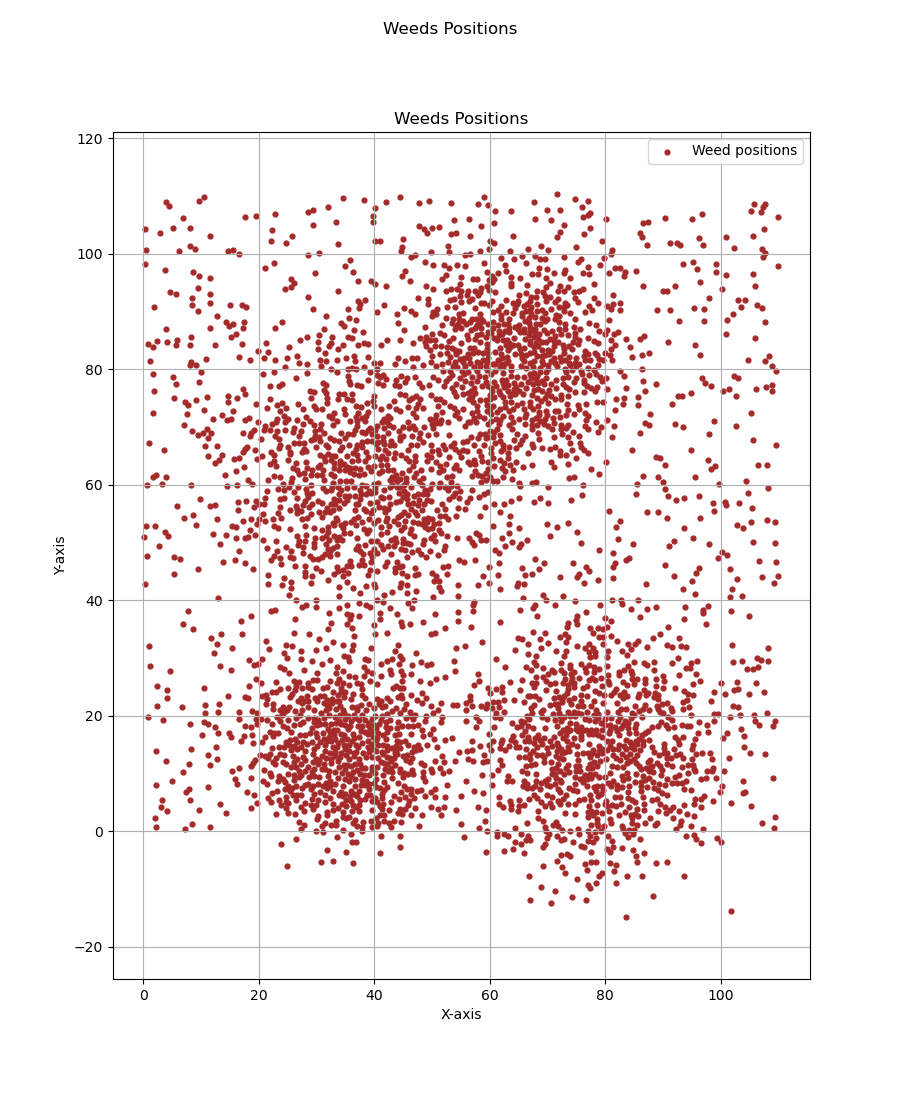
\includegraphics[height=36mm,width=0.24\textwidth]{Images/data/42.png}
% % % %         & 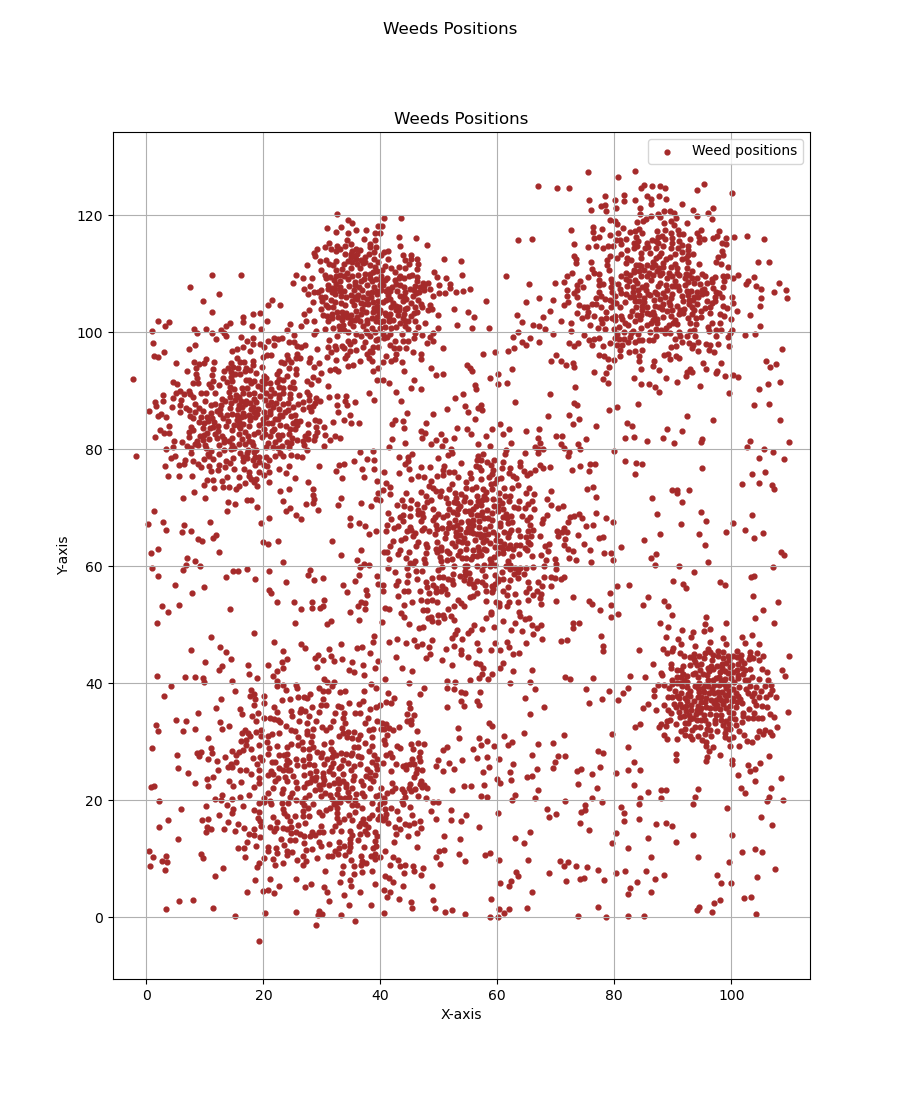
\includegraphics[height=36mm,width=0.24\textwidth]{Images/data/43.png}
% % % %         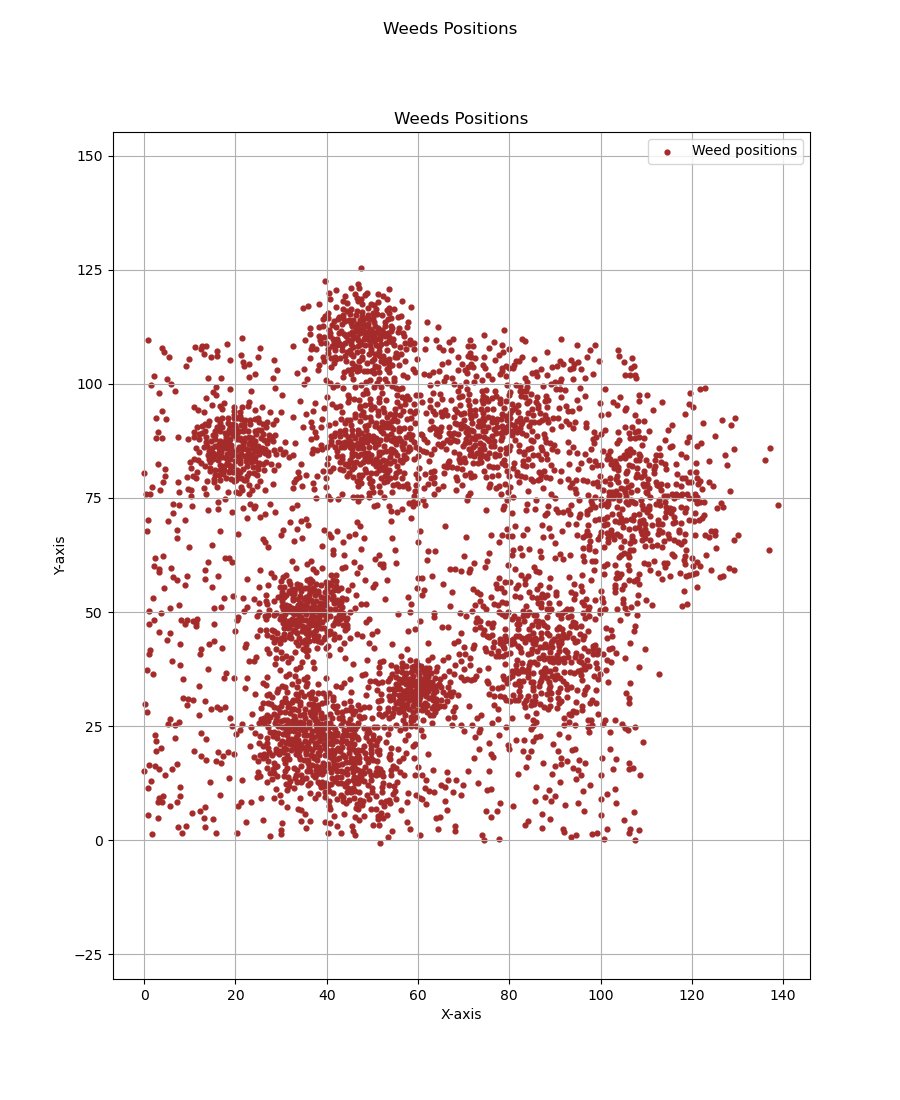
\includegraphics[height=36mm,width=0.24\textwidth]{Images/data/44.png}\\[-4pt]

% % % %         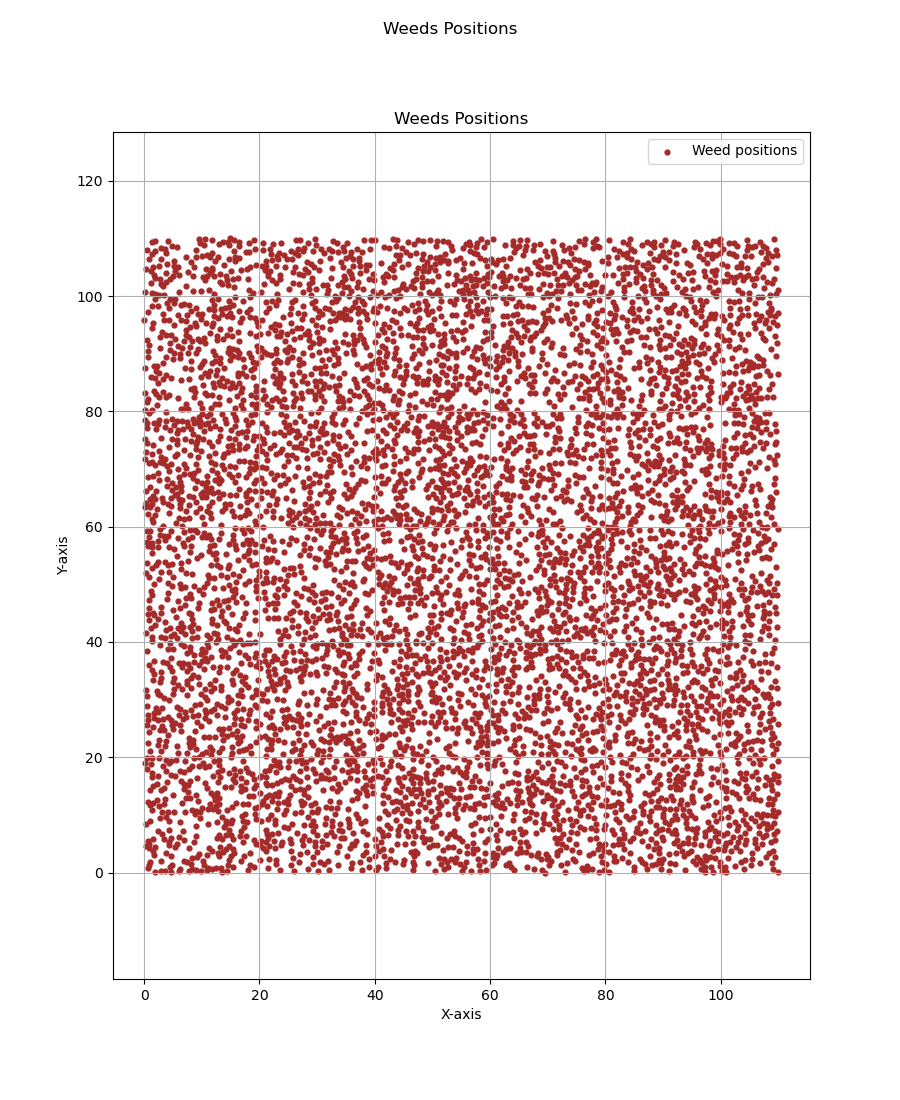
\includegraphics[height=36mm,width=0.24\textwidth]{Images/data/51.png}
% % % %         & 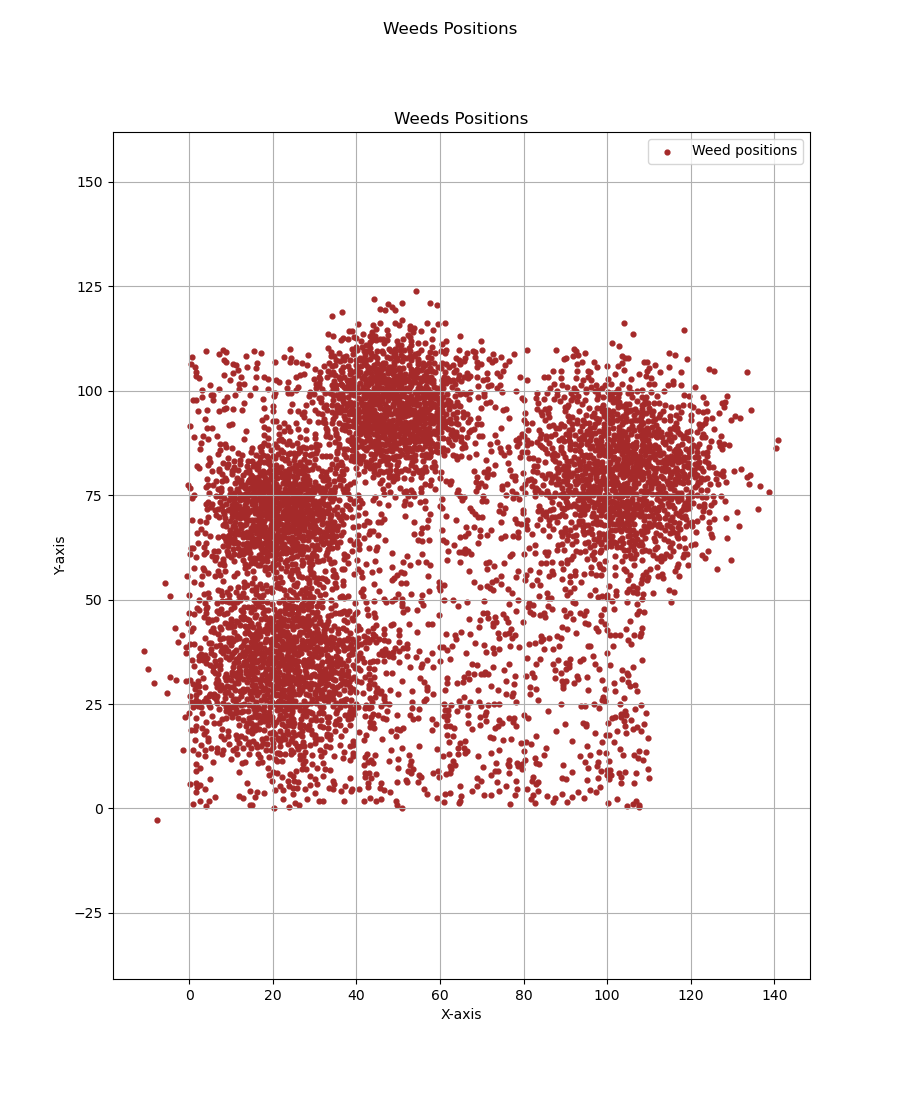
\includegraphics[height=36mm,width=0.24\textwidth]{Images/data/52.png}
% % % %         & 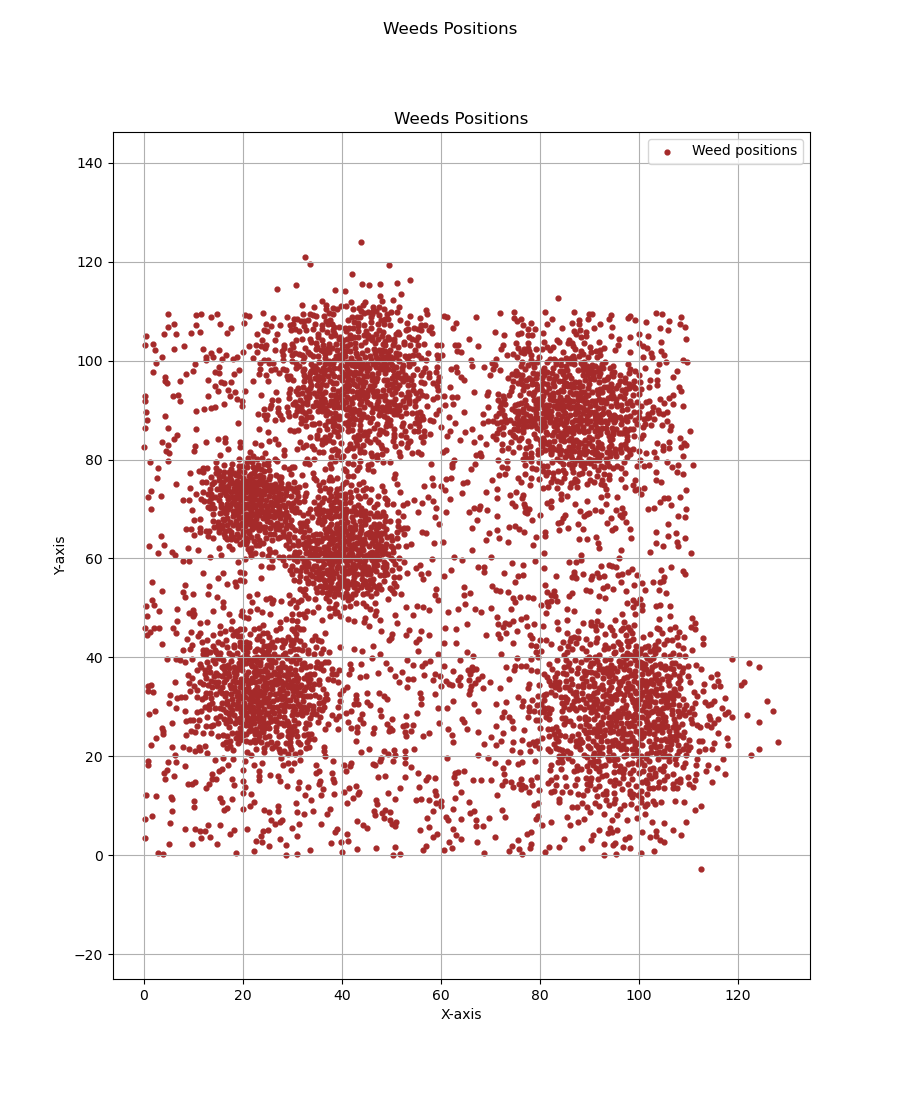
\includegraphics[height=36mm,width=0.24\textwidth]{Images/data/53.png}
% % % %         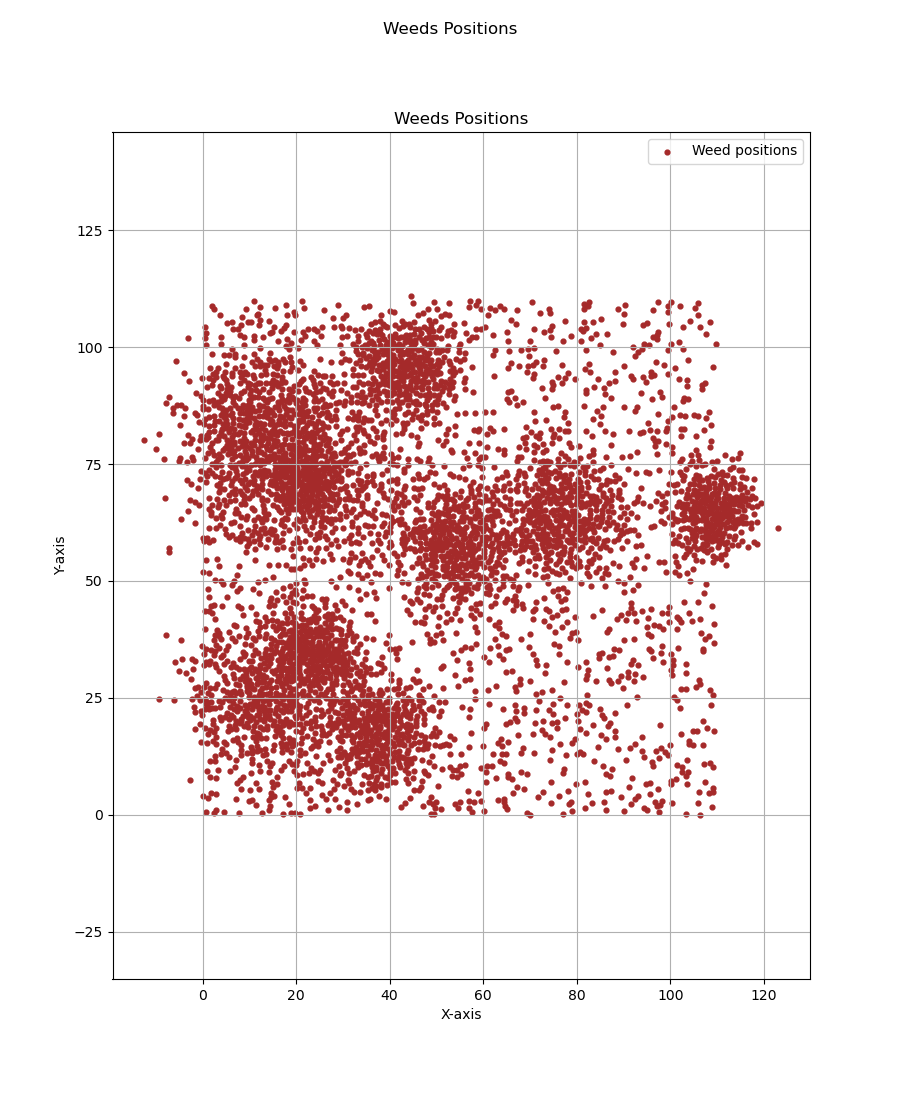
\includegraphics[height=36mm,width=0.24\textwidth]{Images/data/54.png}\\[-4pt]
        
% % % %     \end{tabular}
% % % %     \caption{Dataset.\label{fig:Dataset}}
% % % % \end{figure}


\subsection{Simulation Results and Analysis}

This section presents the detailed results and analysis of the simulation experiments conducted to evaluate the robustness of the proposed complete coverage path planning behavioral algorithm. The empirical findings are meticulously analyzed to provide insights into the algorithm's performance under diverse scenarios, enabling a comprehensive assessment of its efficiency and effectiveness. 

\vspace*{6mm}  

\textbf{Experimental Consistency}
To ensure the validity of comparisons and isolate the effects of different datasets on the algorithm's performance, the initial position and orientation of the robot were kept constant throughout all experiments. Additionally, the parameters for both the robot and the algorithm were consistently maintained across all trials.


\vspace*{6mm}  

\textbf{Robot Constraints and Algorithm Parameters: } 


The robot's constraints and operational parameters are set to realistic values to ensure the validity of the simulation results. The parameters' data can be visualized in (\autoref{tab:constraints_and_parameters_1}), offering a comprehensive overview of the robot's physical and operational characteristics.

% % % % % Table robot parameters 1
% % % % \begin{table}[H] 
% % % %     \centering
% % % %     \caption{Robot and algorithm Constraints and Parameters}
% % % %     \label{tab:constraints_and_parameters_1}
% % % %     \begin{tabular}{|c|c|}
% % % %     \hline
% % % %     \rowcolor[HTML]{FFCC67} 
% % % %     \textit{\textbf{Constraints and Parameters}}                                    & \textit{\textbf{Values}} \\ \hline
% % % %     \rowcolor[HTML]{BBF6F4} 
% % % %     \textit{Robot initial position}                                                 & {[}60.0, 1.0{]}          \\ \hline
% % % %     \rowcolor[HTML]{BBF6F4} 
% % % %     \textit{Robot initial orientation}                                              & 120                      \\ \hline
% % % %     \rowcolor[HTML]{BBF6F4} 
% % % %     \textit{Search angle of the vision cone}                                        & ±11                      \\ \hline
% % % %     \rowcolor[HTML]{BBF6F4} 
% % % %     \textit{Minimum search radius of the vision cone.}                              & 1.25                     \\ \hline
% % % %     \rowcolor[HTML]{BBF6F4} 
% % % %     \textit{Maximum search radius of the vision cone.}                              & 100                      \\ \hline
% % % %     \rowcolor[HTML]{BBF6F4} 
% % % %     \textit{Minimum turning radius allowed for the robot.}                          & 2.0                      \\ \hline
% % % %     \rowcolor[HTML]{BBF6F4} 
% % % %     \textit{robot velocity on curved paths.}                                        & 0.4                      \\ \hline
% % % %     \rowcolor[HTML]{BBF6F4} 
% % % %     \textit{robot velocity on straight paths.}                                      & 0.8                      \\ \hline
% % % %     \rowcolor[HTML]{BBF6F4} 
% % % %     \textit{Distance used to compute field time taken on curved paths.}             & 7.85                     \\ \hline
% % % %     \rowcolor[HTML]{BBF6F4} 
% % % %     \textit{Number of points to consider in the vision cone.}                       & 5                        \\ \hline
% % % %     \rowcolor[HTML]{BEF7F5} 
% % % %     \textit{Minimum distance between intermediate points, and start and end point.} & 2.7                      \\ \hline
% % % %     \rowcolor[HTML]{BEF7F5} 
% % % %     \textit{Minimum distance between intermediate points.}                          & 2                        \\ \hline
% % % %     \rowcolor[HTML]{BEF7F5} 
% % % %     \textit{Maximum distance of the point form the path.}                           & 0.6                      \\ \hline
% % % %     \end{tabular}
% % % %     \end{table}



\vspace*{6mm}   







The algorithm parameters are also meticulously defined to ensure consistent performance across all experiments. These parameters are set based on the robot's physical constraints and operational requirements, ensuring that the algorithm operates within realistic boundaries.

\vspace*{6mm}

The algorithm was designed to initially compute the global coverage path using straight lines. Subsequently, Dubins paths are generated for each line segment to ensure the shortest feasible path between each pair of points, optimizing the overall path length. The (\autoref{fig:straight_path}) illustrate the straight paths generated by the algorithm for different datasets.

% % % % % Straight_path
% % % % \begin{figure}[p]
% % % %     \centering
% % % %     \begin{tabular}{ccc}
% % % %          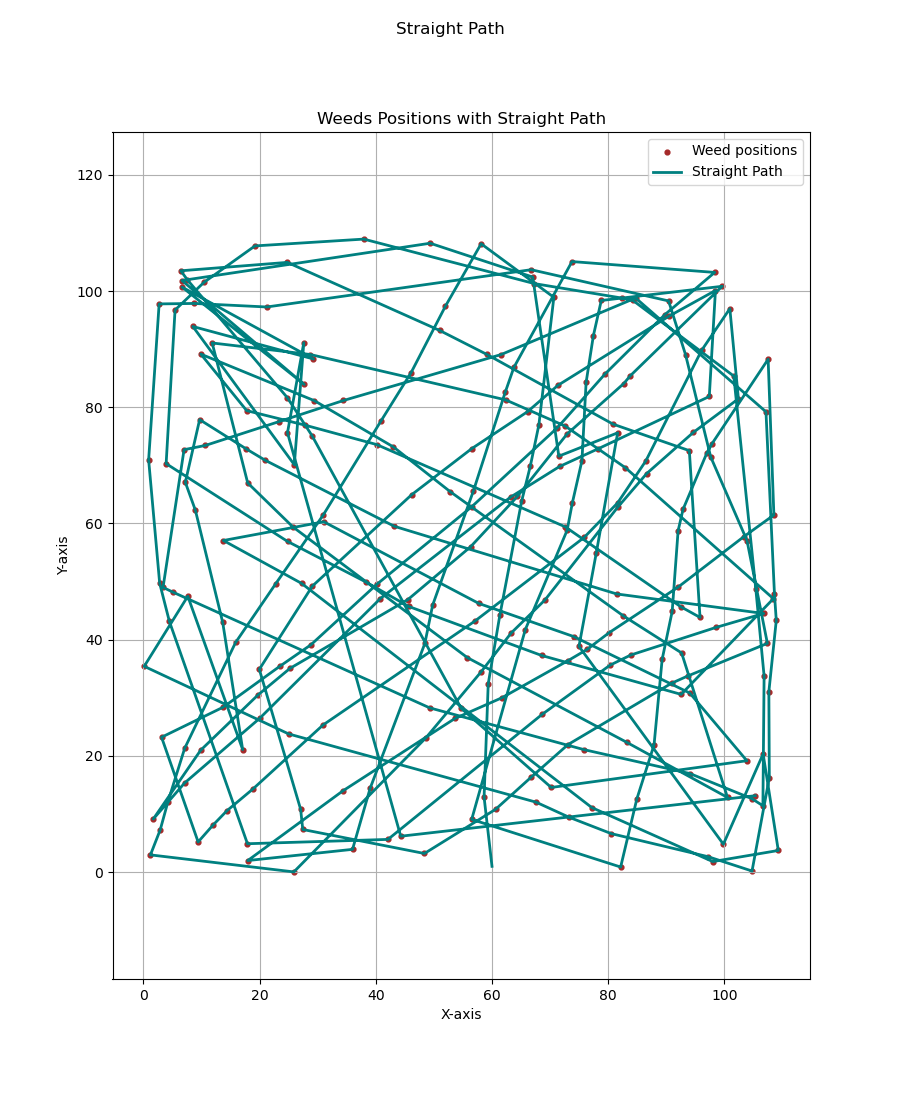
\includegraphics[height=36mm,width=0.24\textwidth]{Images/simulation_no_obs/straight_paths/01.png}
% % % %         & 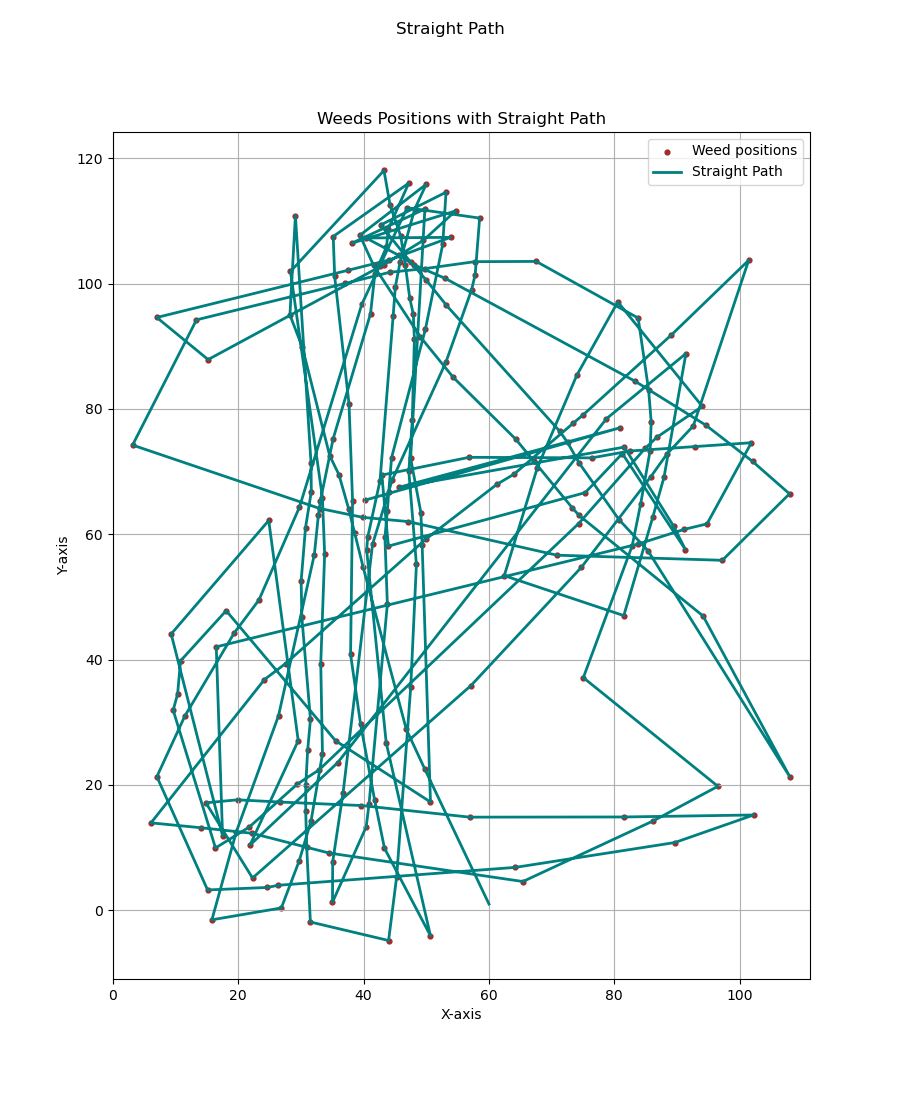
\includegraphics[height=36mm,width=0.24\textwidth]{Images/simulation_no_obs/straight_paths/02.png}
% % % %         & 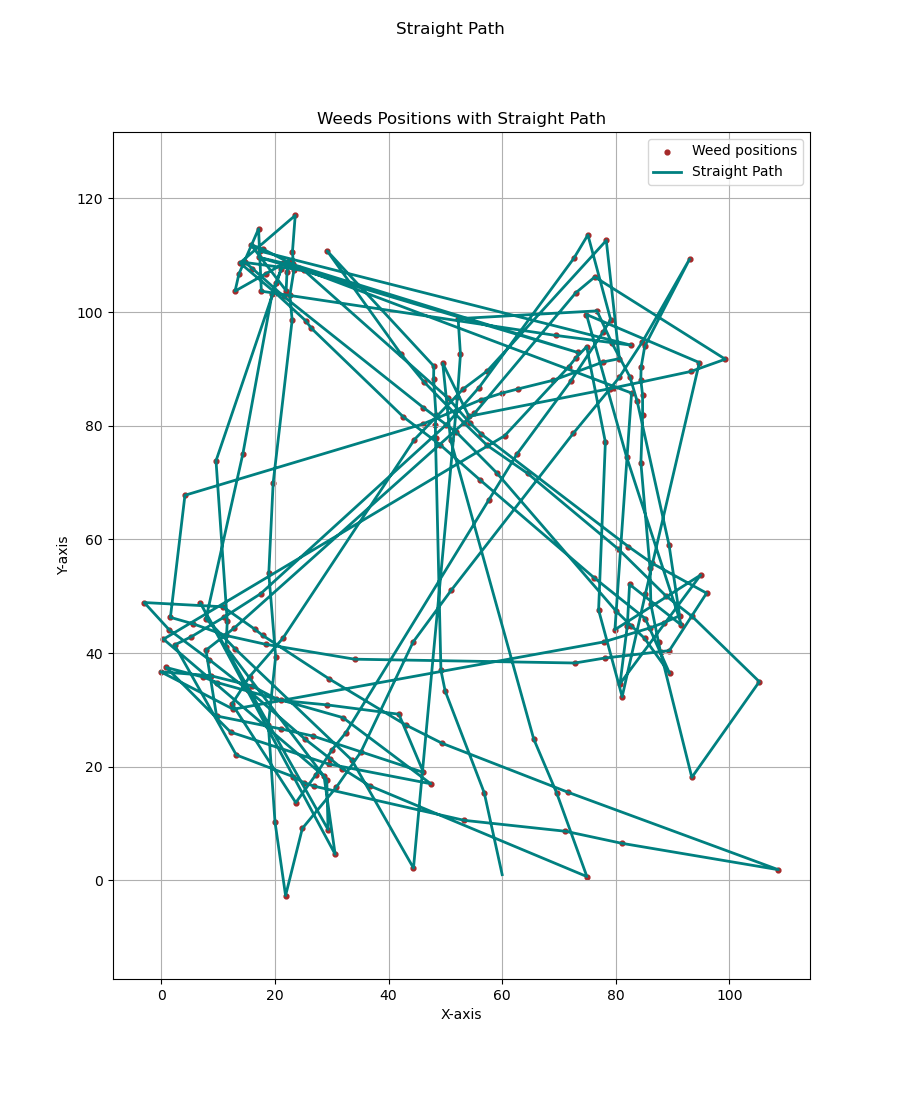
\includegraphics[height=36mm,width=0.24\textwidth]{Images/simulation_no_obs/straight_paths/03.png}
% % % %          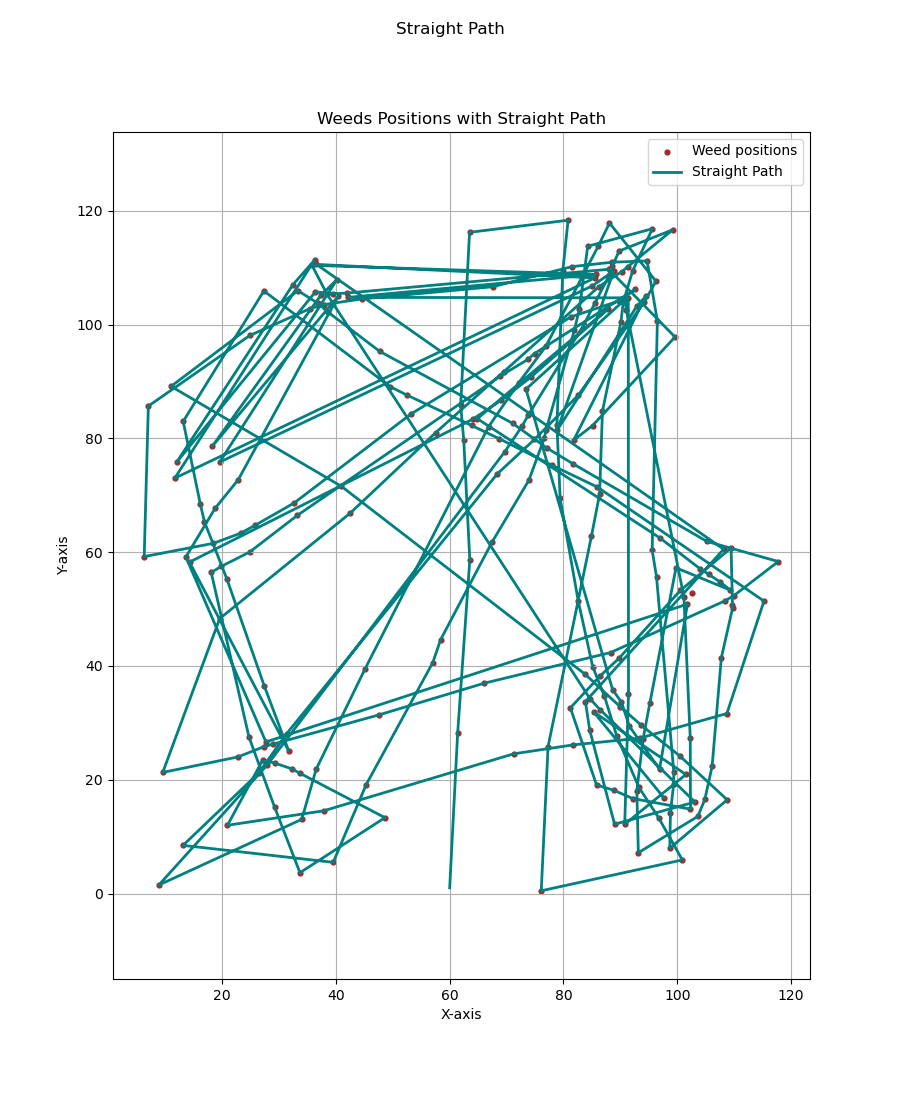
\includegraphics[height=36mm,width=0.24\textwidth]{Images/simulation_no_obs/straight_paths/04.png}\\[-4pt]

% % % %         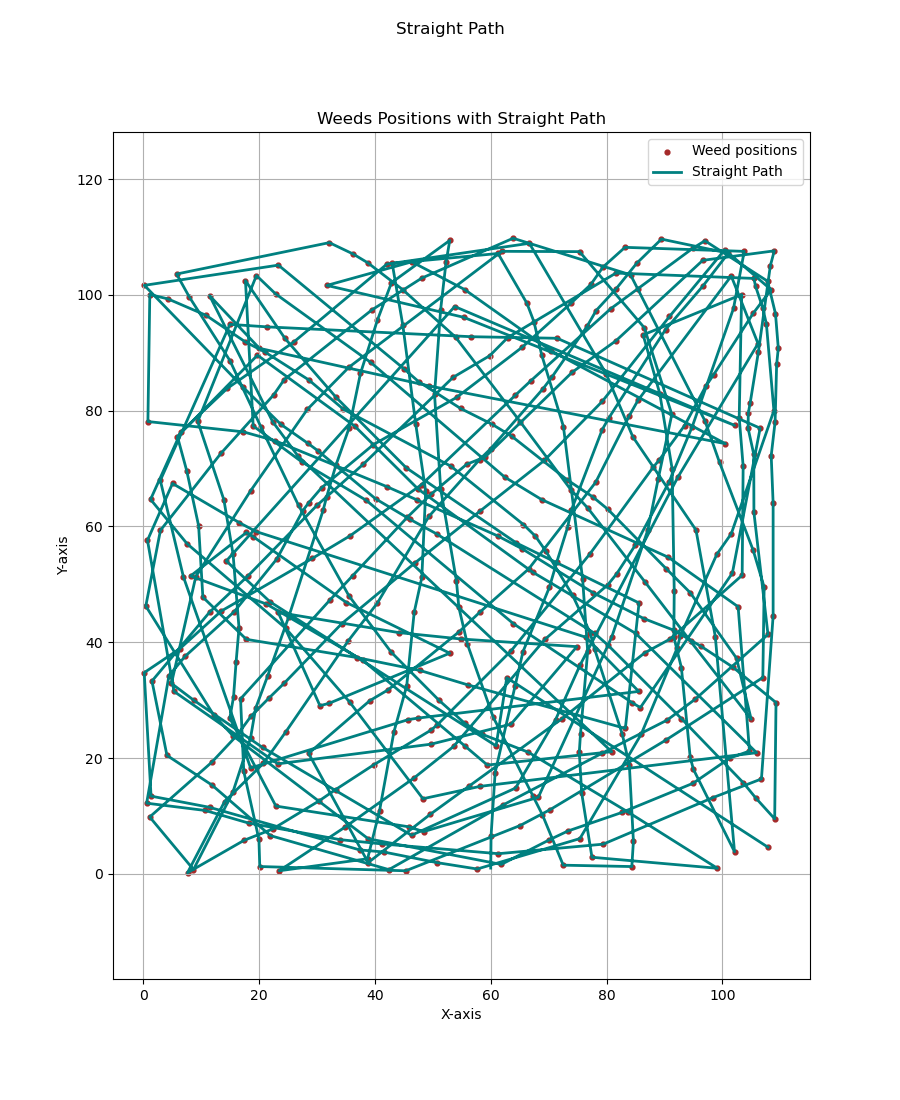
\includegraphics[height=36mm,width=0.24\textwidth]{Images/simulation_no_obs/straight_paths/11.png}
% % % %         & 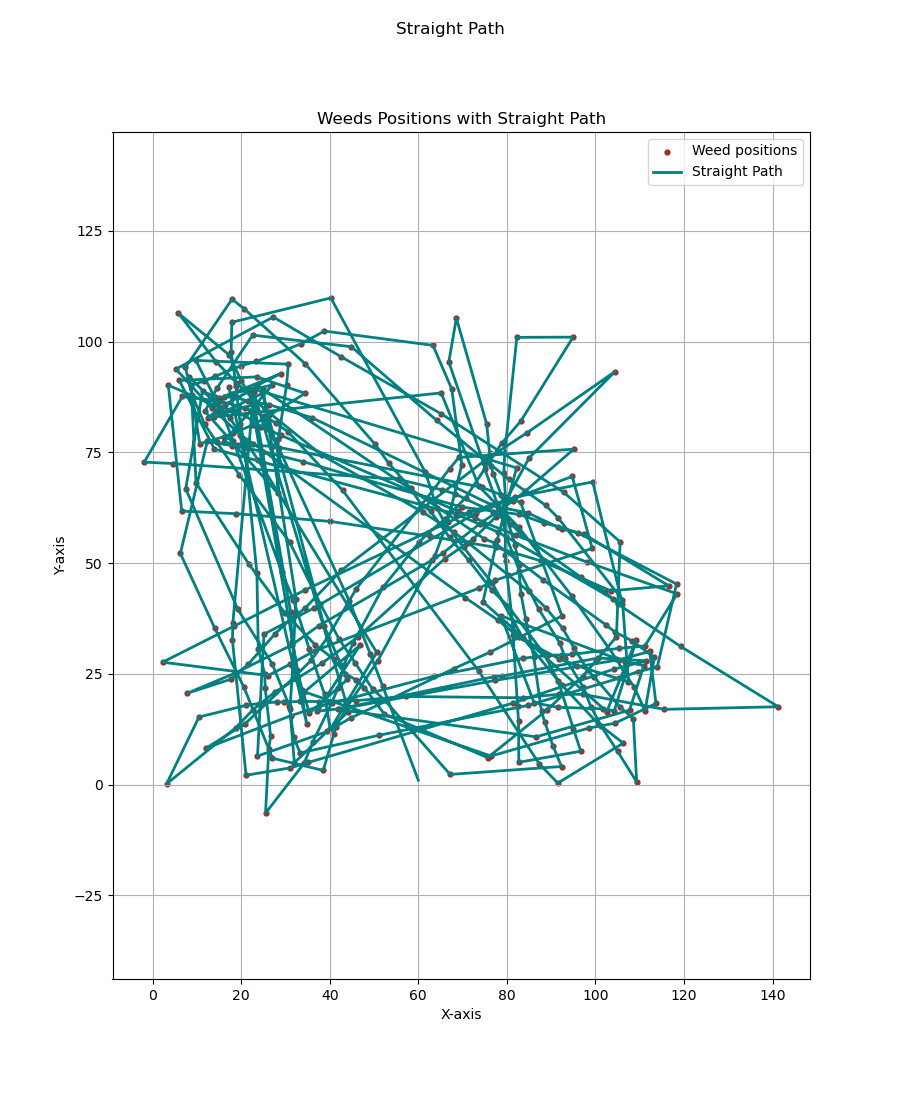
\includegraphics[height=36mm,width=0.24\textwidth]{Images/simulation_no_obs/straight_paths/12.png}
% % % %         & 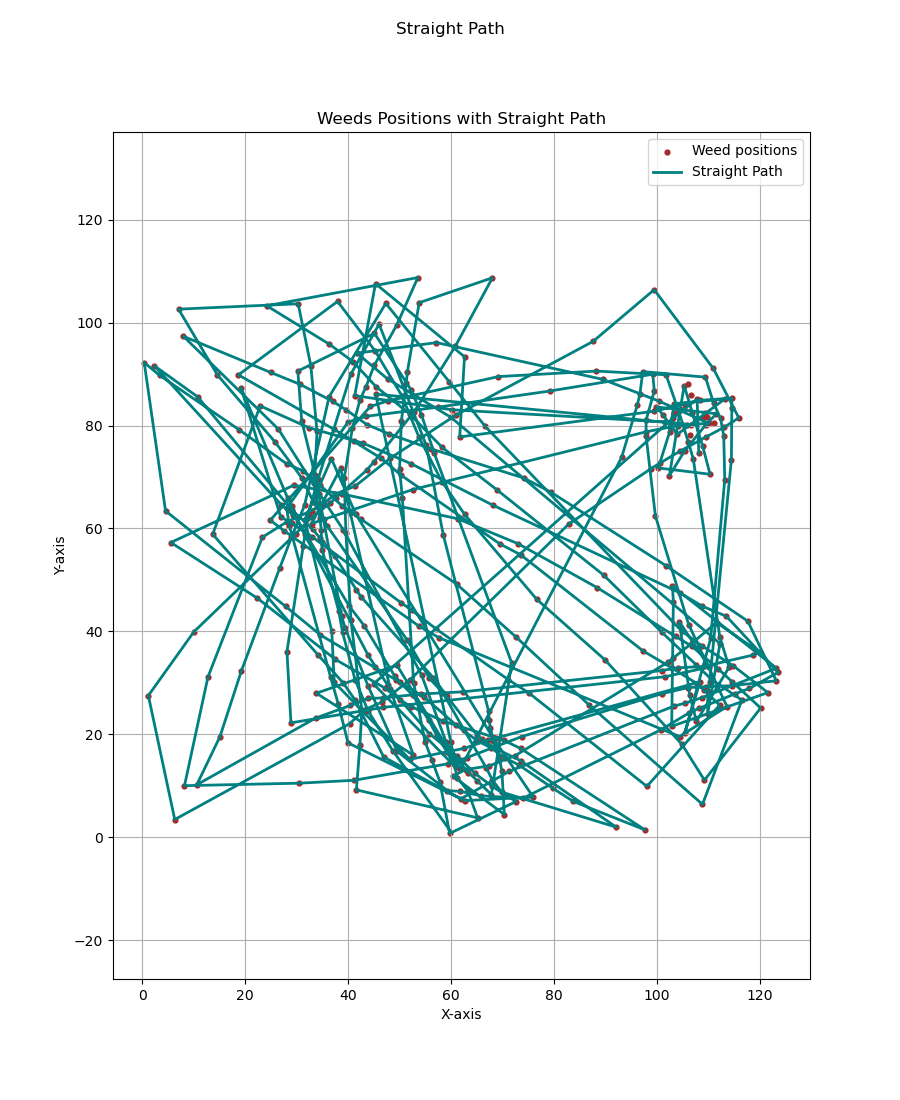
\includegraphics[height=36mm,width=0.24\textwidth]{Images/simulation_no_obs/straight_paths/13.png}
% % % %         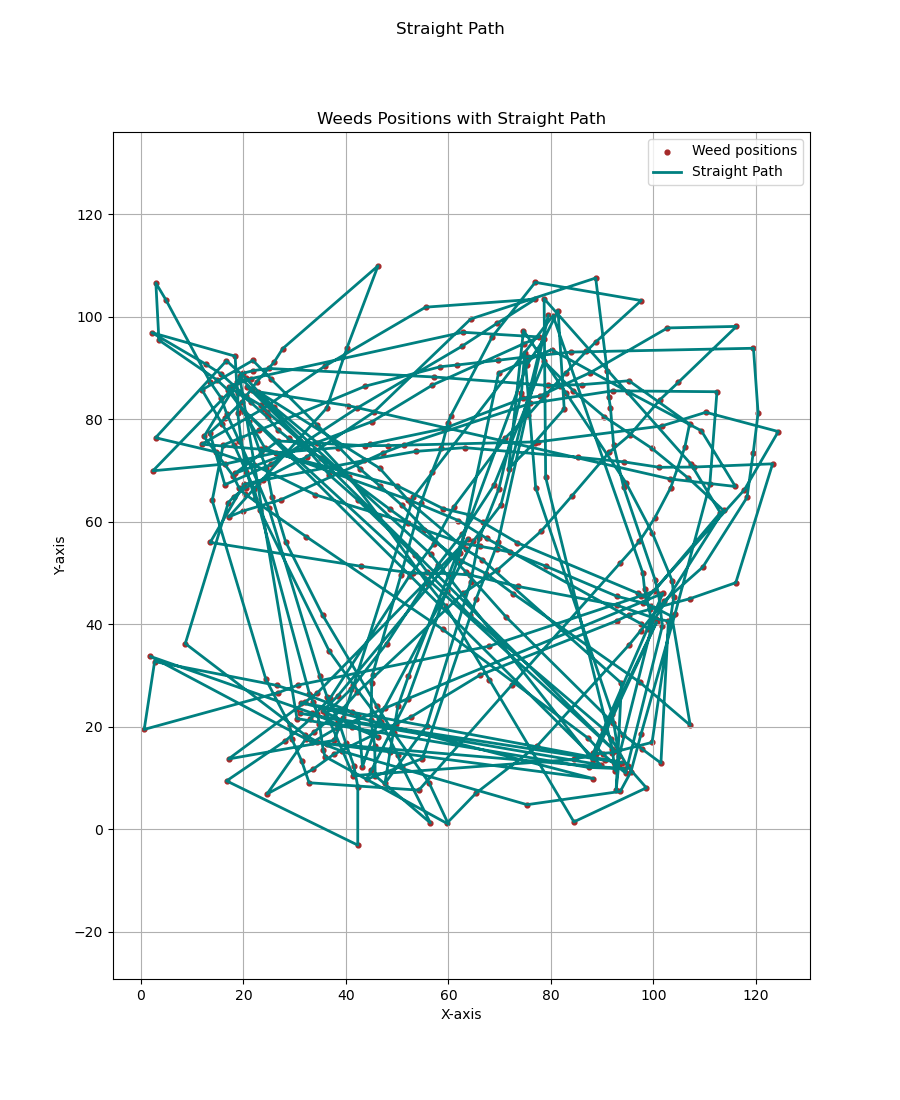
\includegraphics[height=36mm,width=0.24\textwidth]{Images/simulation_no_obs/straight_paths/14.png}\\[-4pt]

% % % %         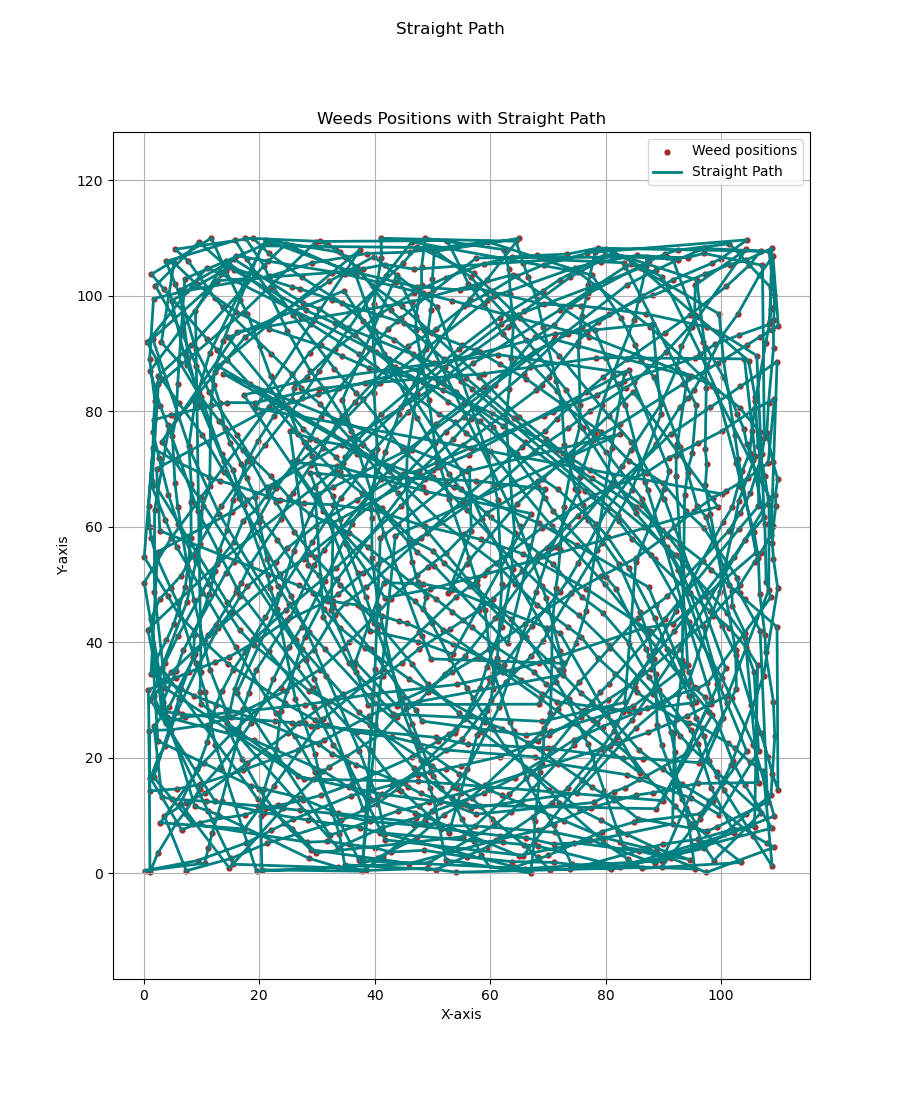
\includegraphics[height=36mm,width=0.24\textwidth]{Images/simulation_no_obs/straight_paths/21.png}
% % % %         & 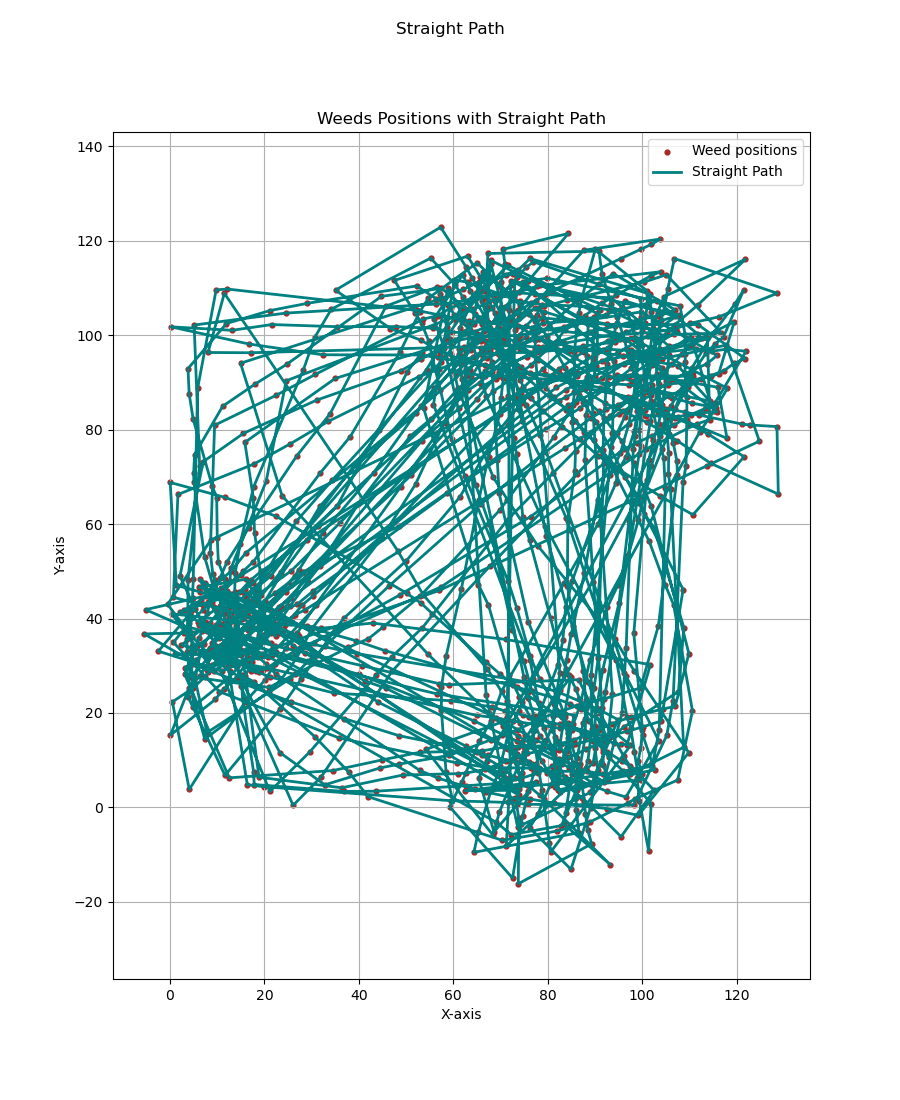
\includegraphics[height=36mm,width=0.24\textwidth]{Images/simulation_no_obs/straight_paths/22.png}
% % % %         & 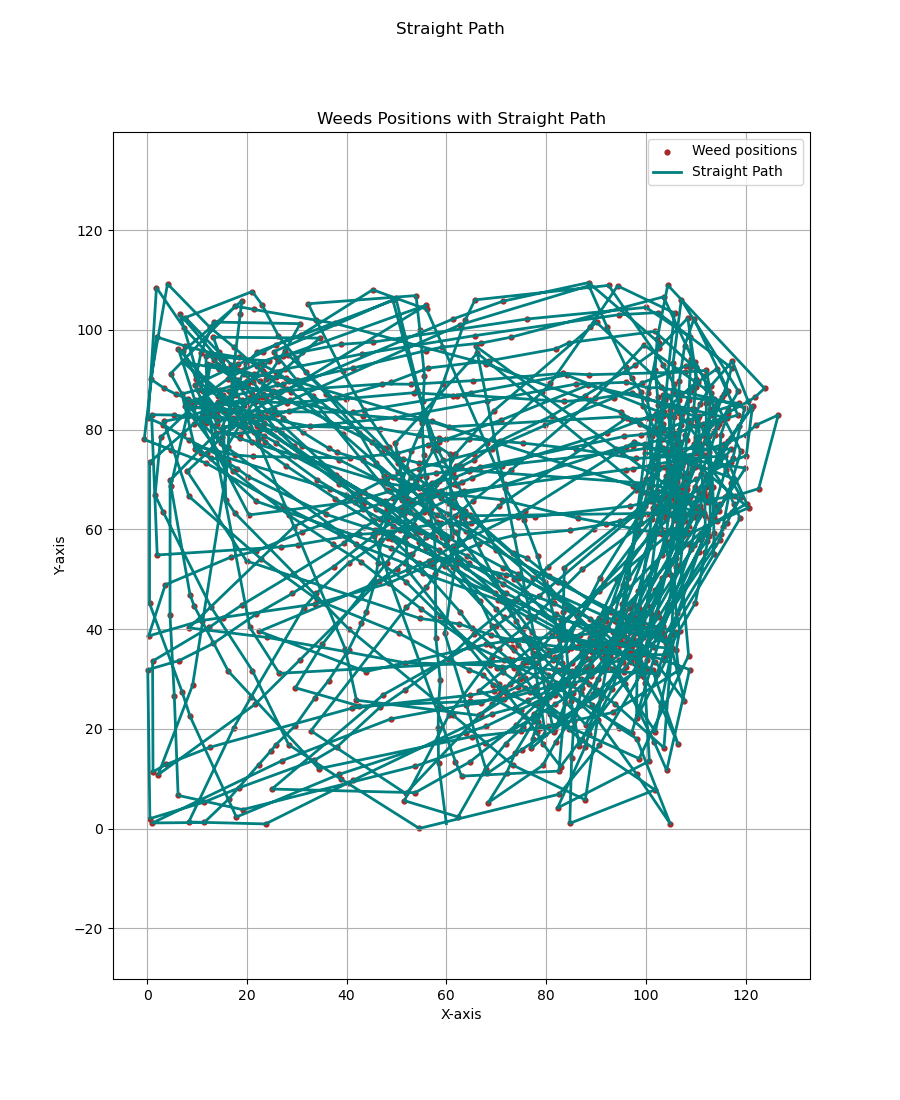
\includegraphics[height=36mm,width=0.24\textwidth]{Images/simulation_no_obs/straight_paths/23.png}
% % % %          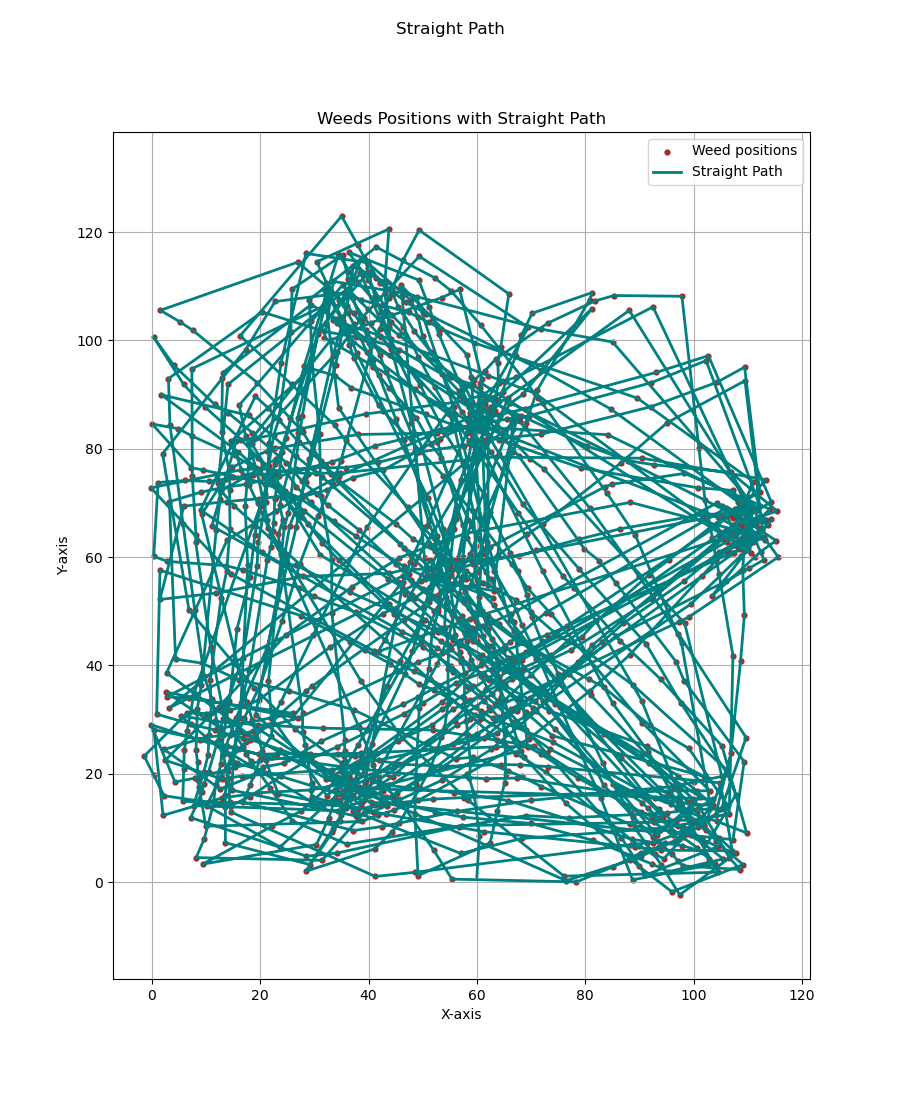
\includegraphics[height=36mm,width=0.24\textwidth]{Images/simulation_no_obs/straight_paths/24.png}\\[-4pt]

% % % %          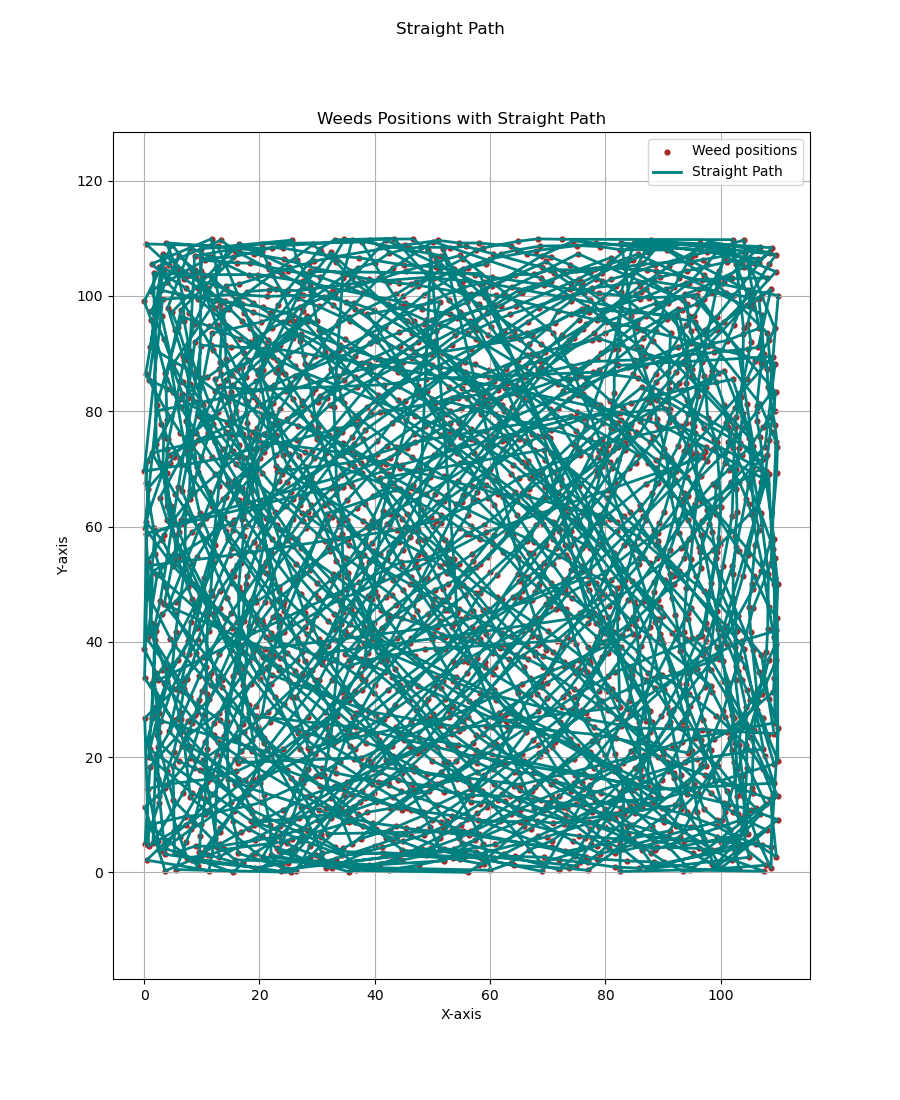
\includegraphics[height=36mm,width=0.24\textwidth]{Images/simulation_no_obs/straight_paths/31.png}
% % % %         & 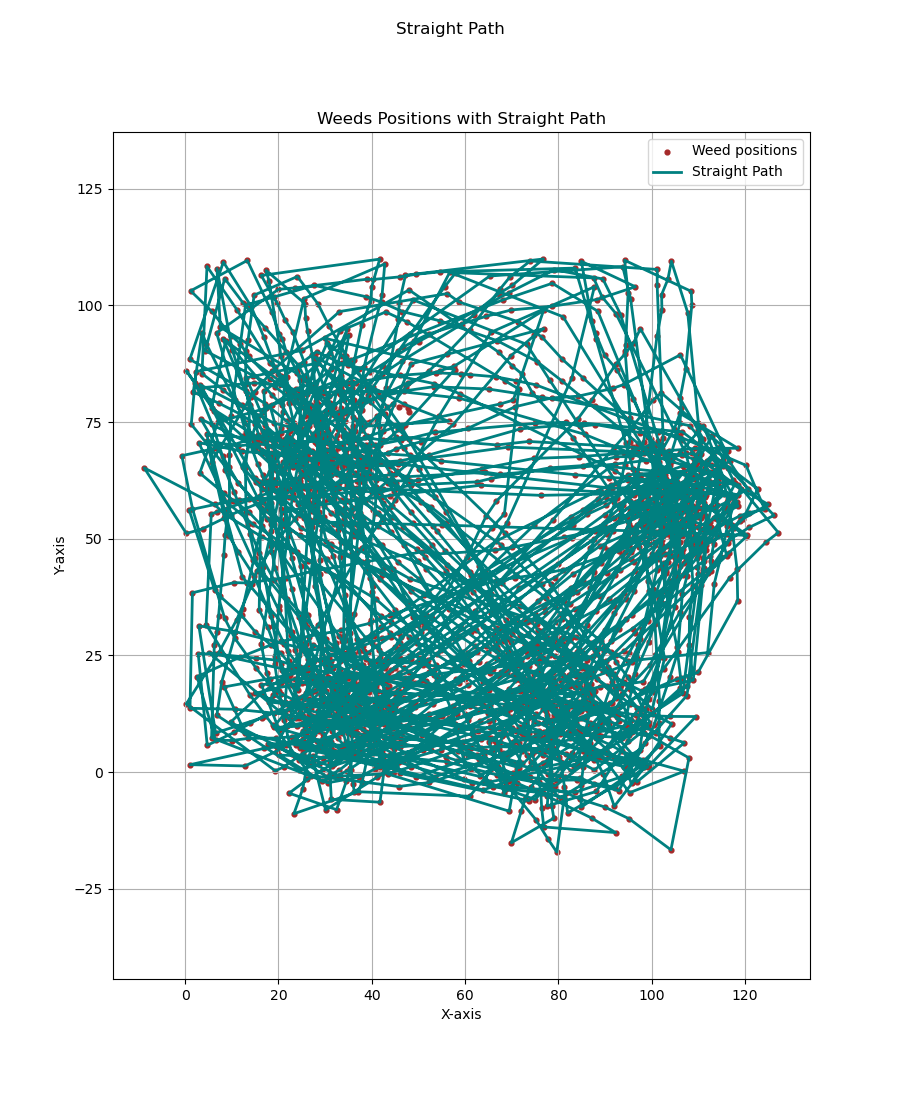
\includegraphics[height=36mm,width=0.24\textwidth]{Images/simulation_no_obs/straight_paths/32.png}
% % % %         & 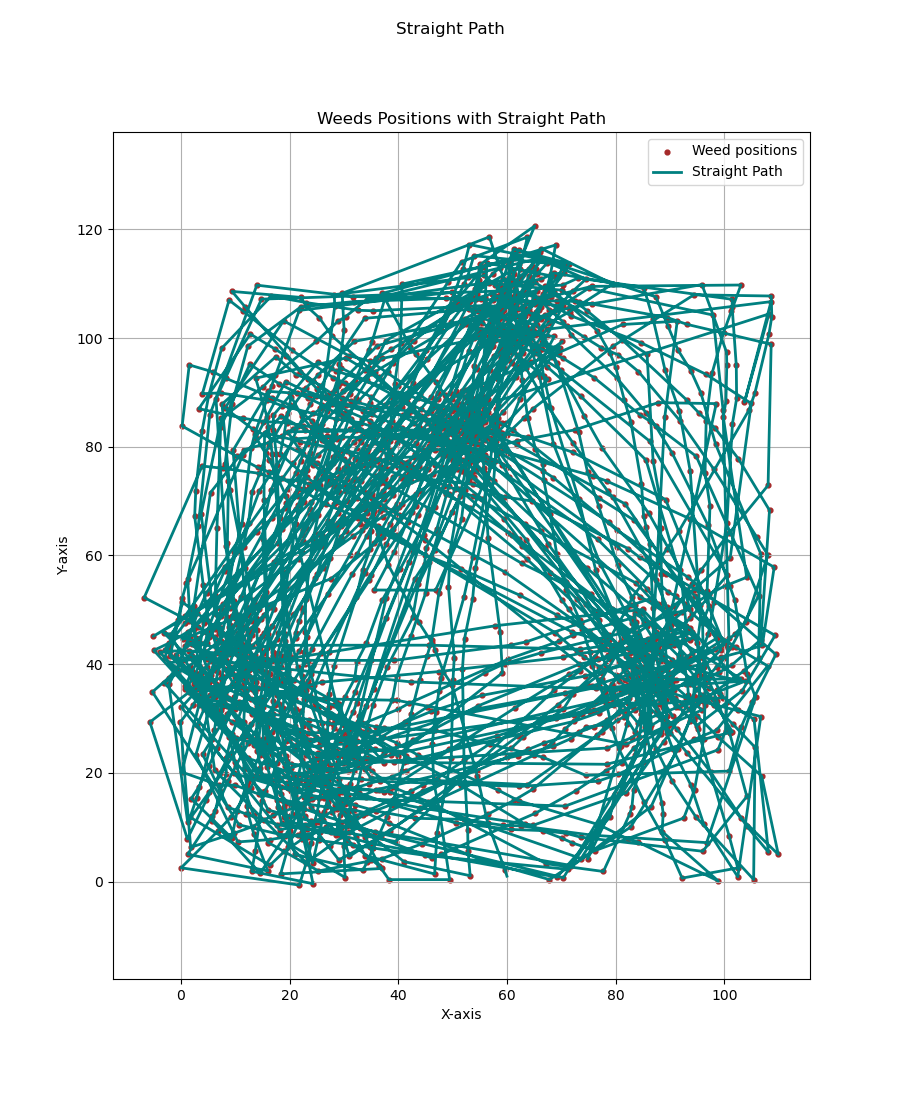
\includegraphics[height=36mm,width=0.24\textwidth]{Images/simulation_no_obs/straight_paths/33.png}
% % % %          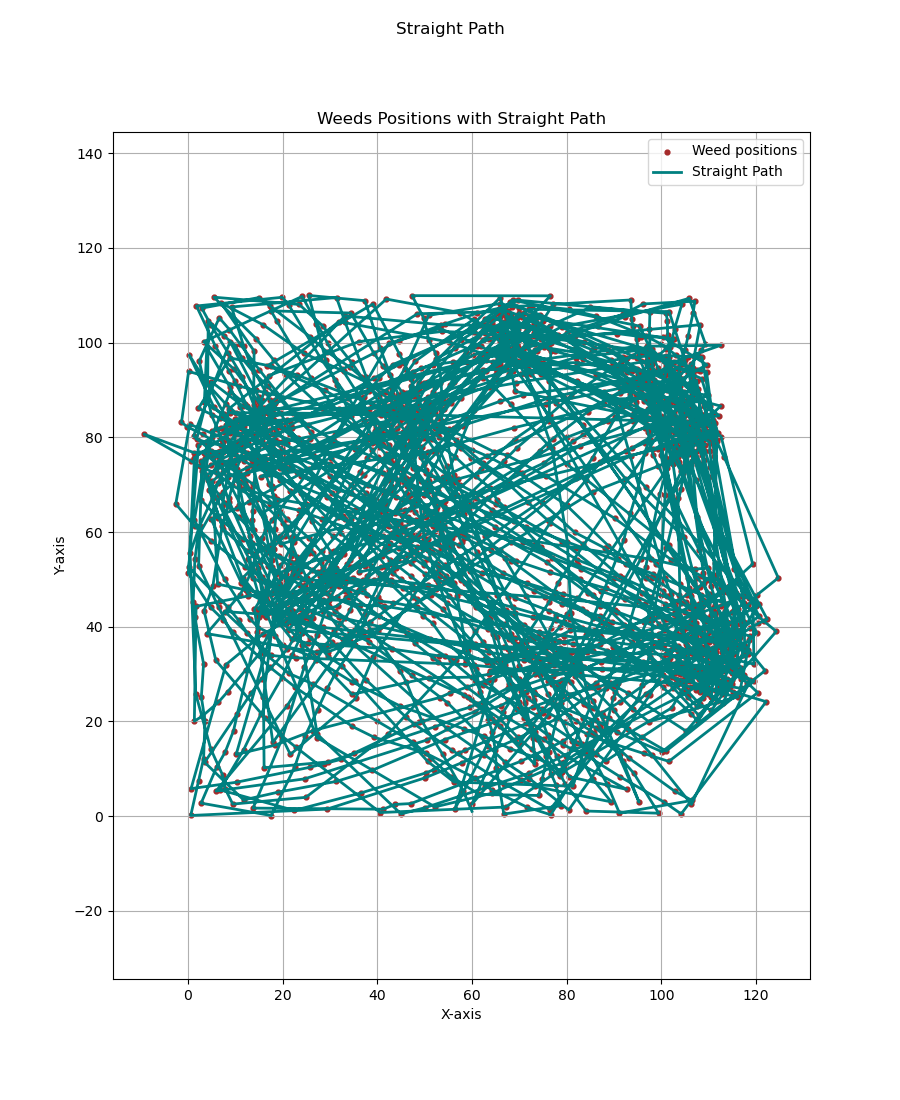
\includegraphics[height=36mm,width=0.24\textwidth]{Images/simulation_no_obs/straight_paths/34.png}\\[-4pt]


% % % %         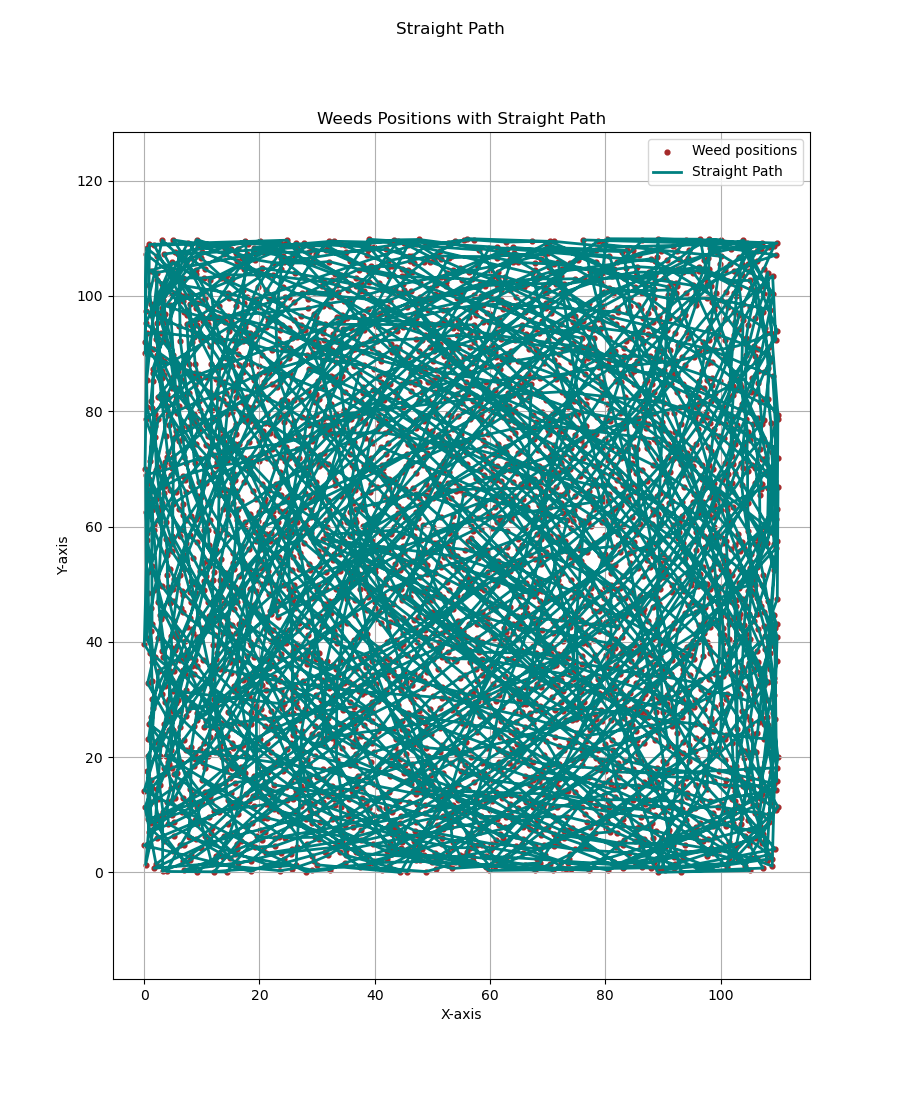
\includegraphics[height=36mm,width=0.24\textwidth]{Images/simulation_no_obs/straight_paths/41.png}
% % % %         & 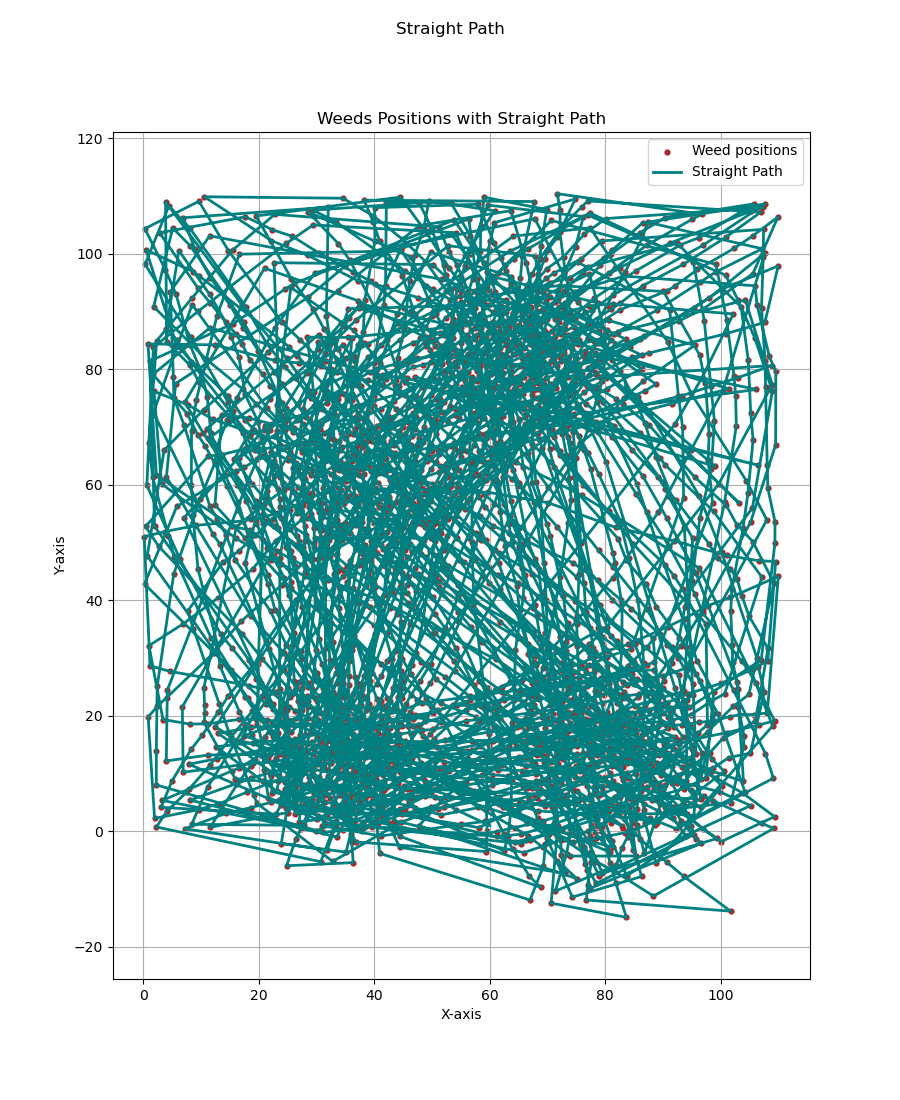
\includegraphics[height=36mm,width=0.24\textwidth]{Images/simulation_no_obs/straight_paths/42.png}
% % % %         & 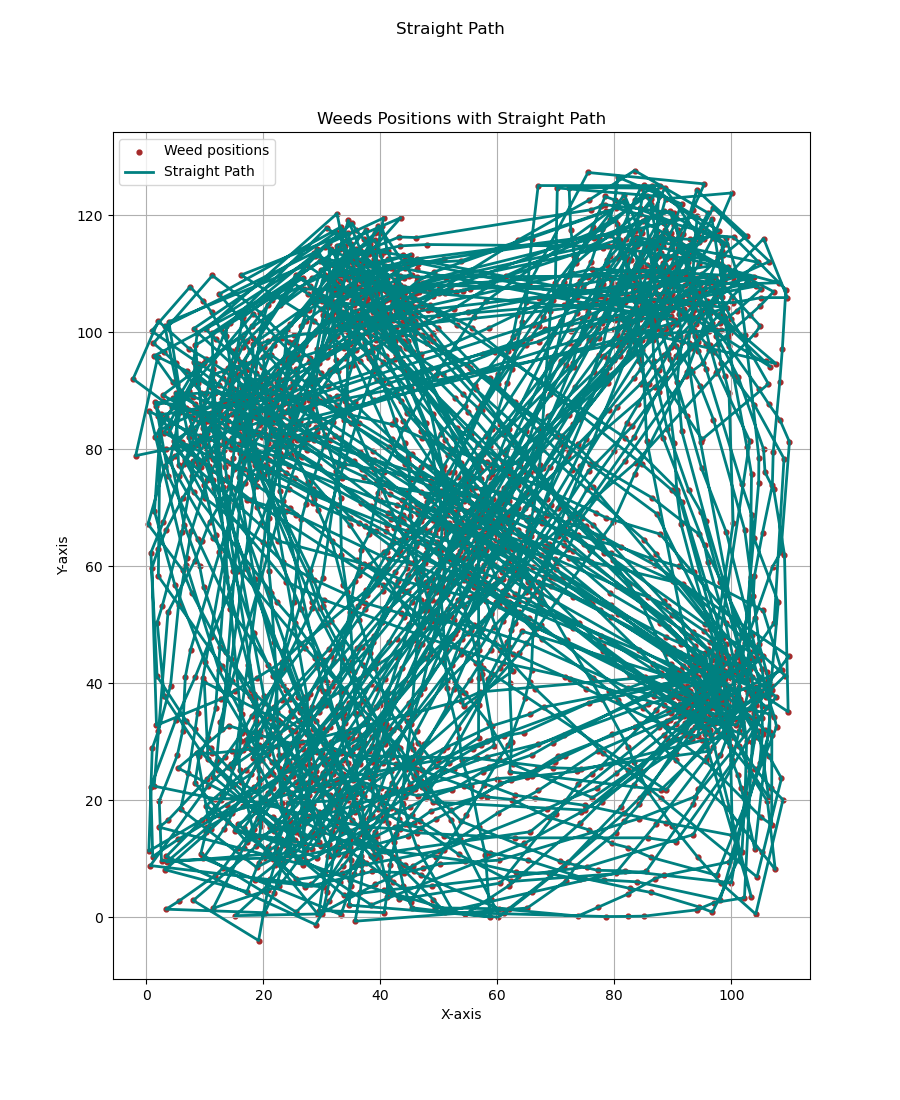
\includegraphics[height=36mm,width=0.24\textwidth]{Images/simulation_no_obs/straight_paths/43.png}
% % % %         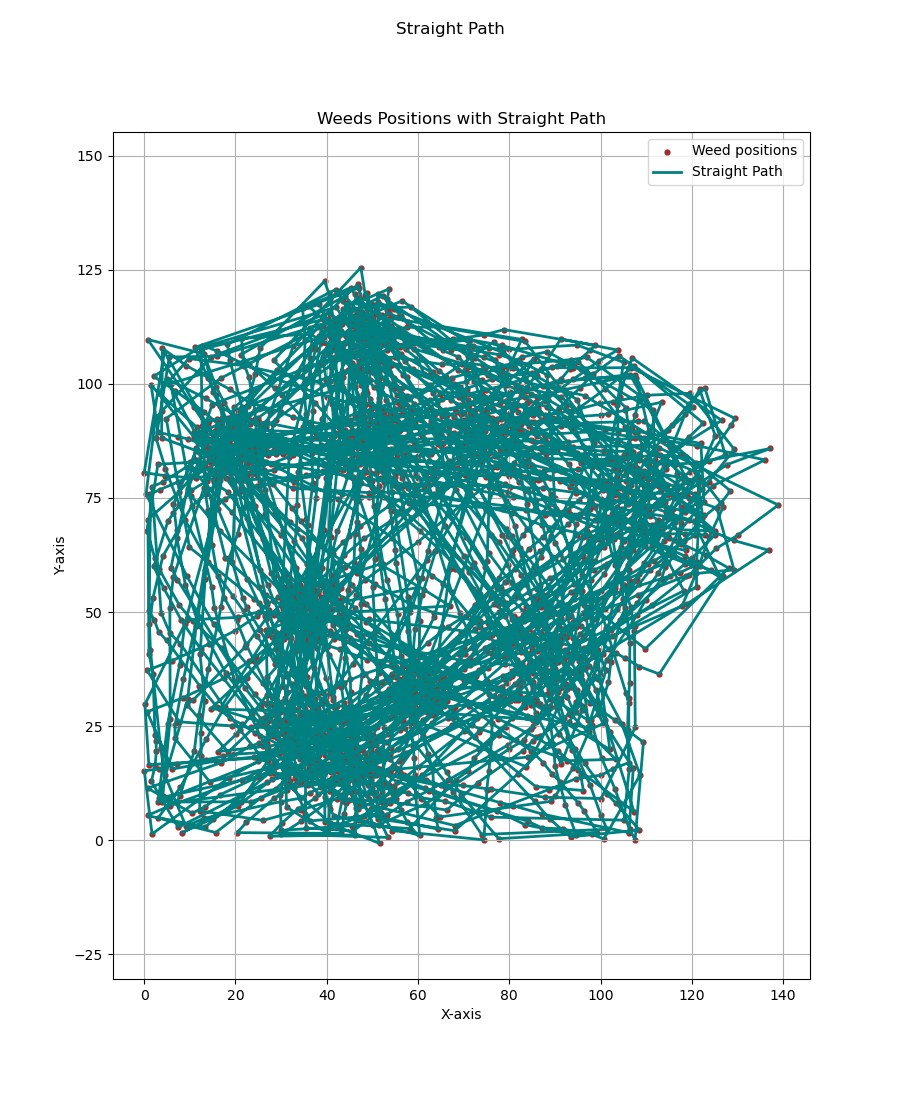
\includegraphics[height=36mm,width=0.24\textwidth]{Images/simulation_no_obs/straight_paths/44.png}\\[-4pt]

% % % %         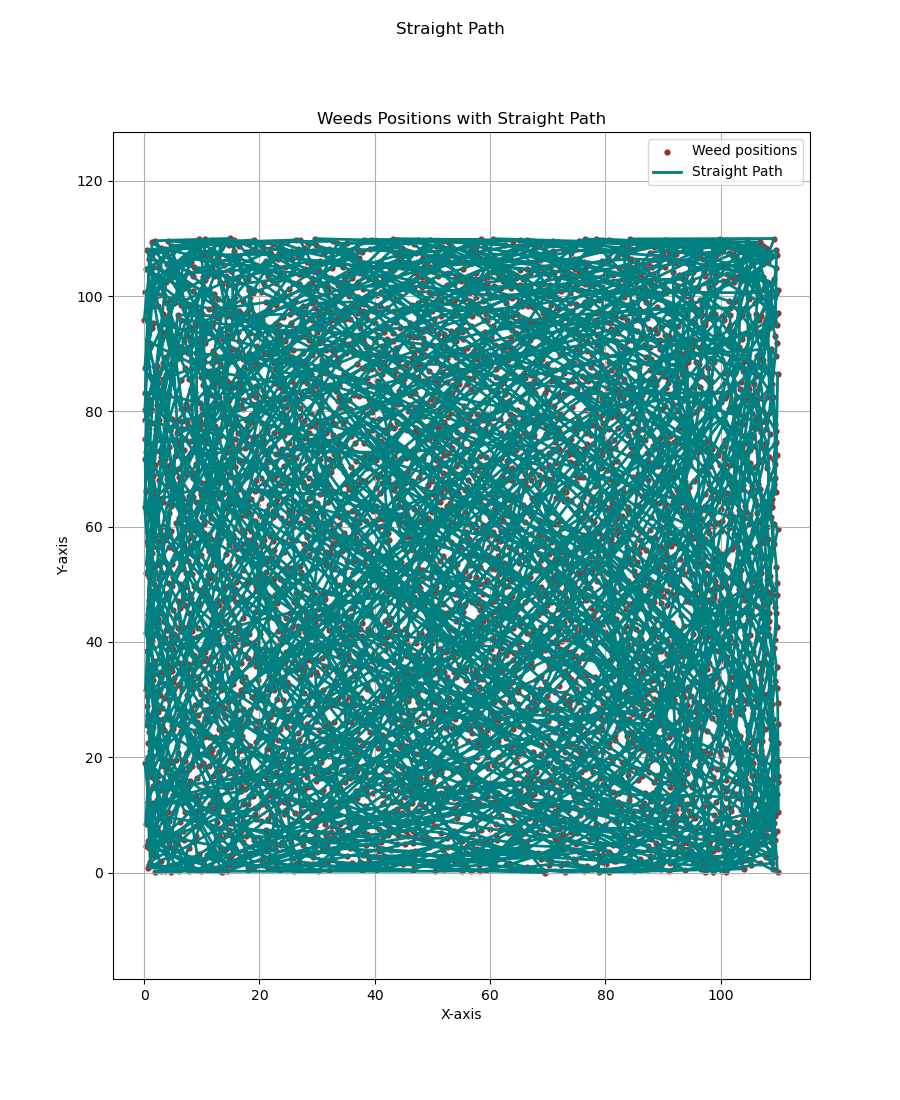
\includegraphics[height=36mm,width=0.24\textwidth]{Images/simulation_no_obs/straight_paths/51.png}
% % % %         & 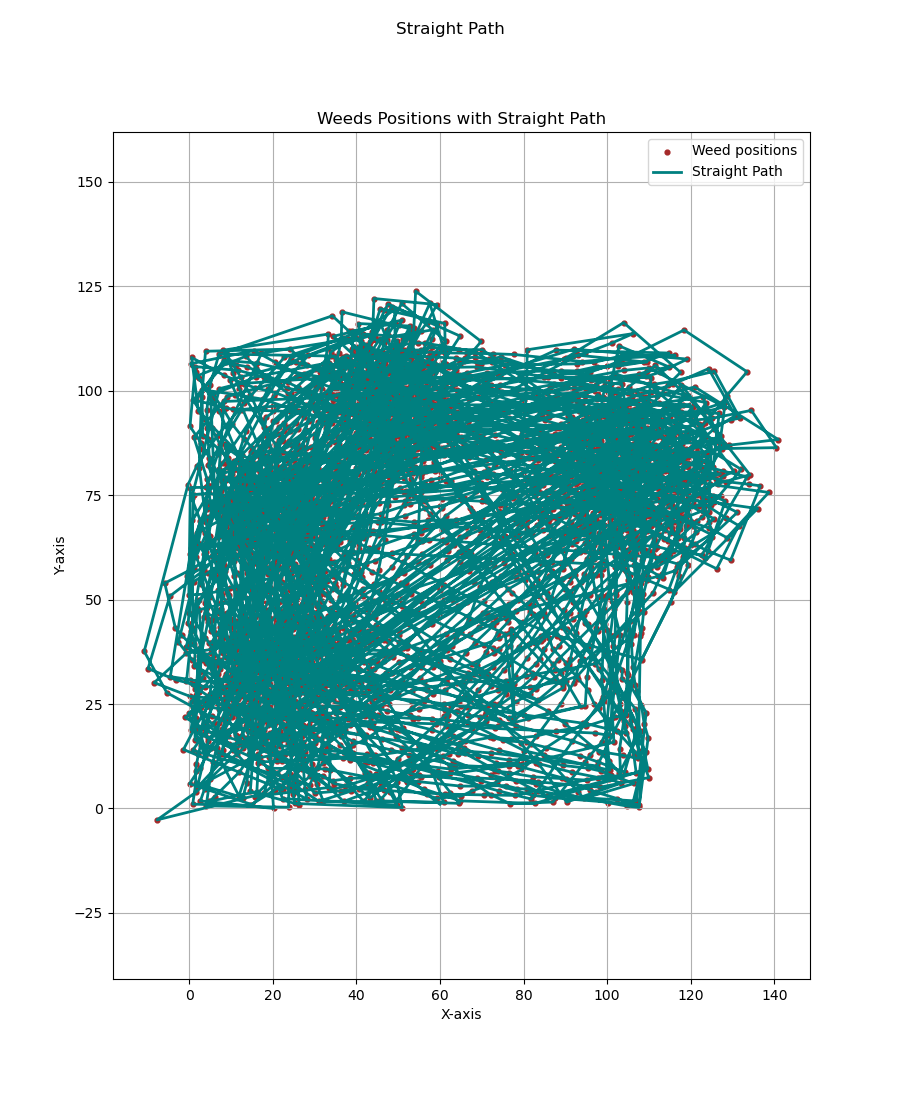
\includegraphics[height=36mm,width=0.24\textwidth]{Images/simulation_no_obs/straight_paths/52.png}
% % % %         & 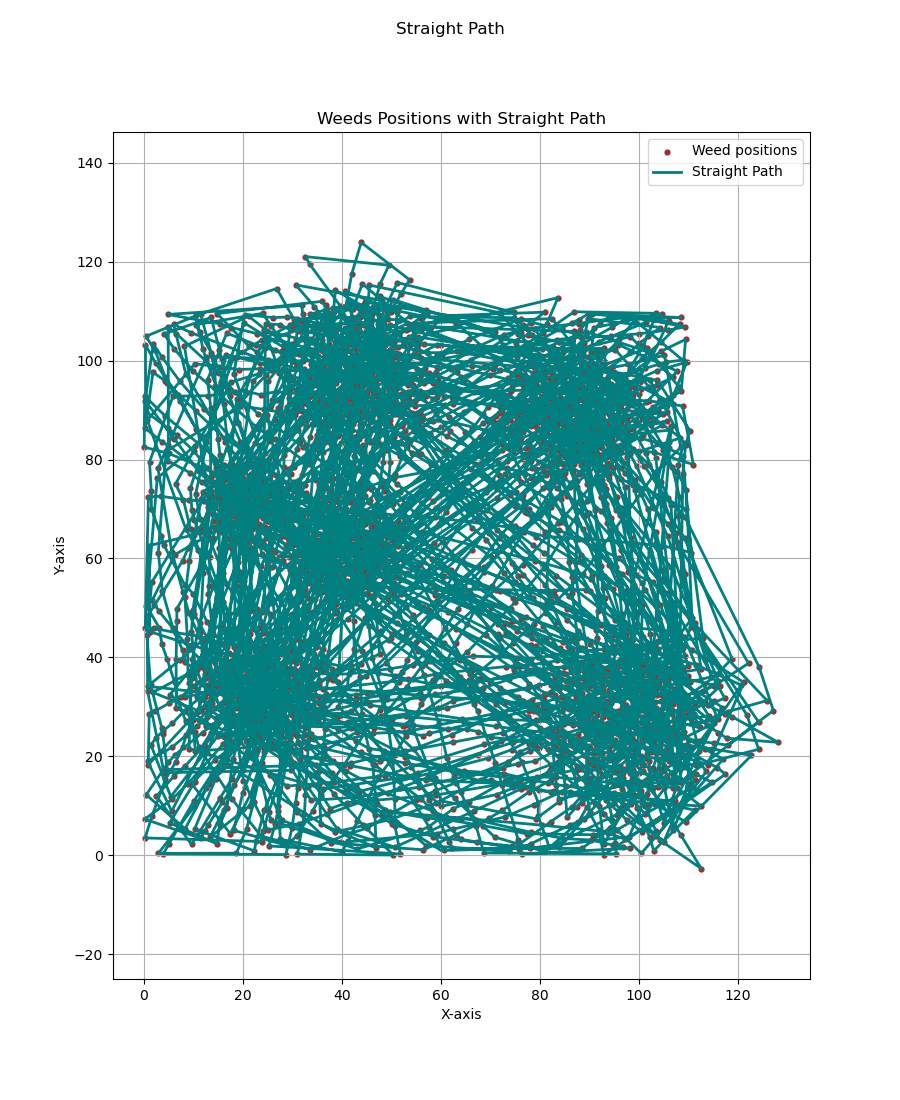
\includegraphics[height=36mm,width=0.24\textwidth]{Images/simulation_no_obs/straight_paths/53.png}
% % % %         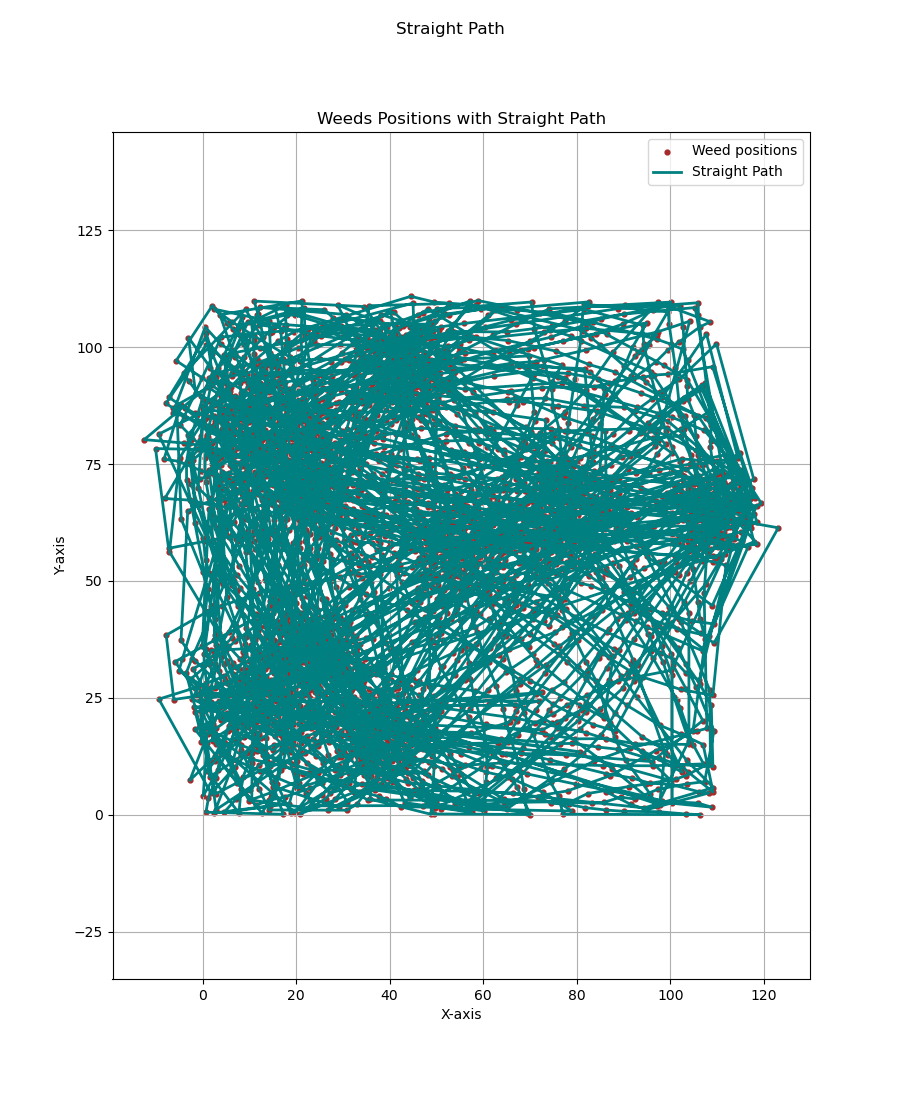
\includegraphics[height=36mm,width=0.24\textwidth]{Images/simulation_no_obs/straight_paths/54.png}\\[-4pt]

% % % %     \end{tabular}
% % % %     \caption{Straight Path.\label{fig:straight_path}}
% % % % \end{figure}


\vspace*{6mm}


Once the Dubins paths are generated from the straight paths, the resultant paths can be visualized in the (\autoref{fig:dubins_path}). These figures showcase the robot's traversal across different datasets, illustrating how the algorithm adapts to various point distributions.
% % % % % Dubin's path
% % % % \begin{figure}[p]
% % % %     \centering
% % % %     \begin{tabular}{ccc}
% % % %          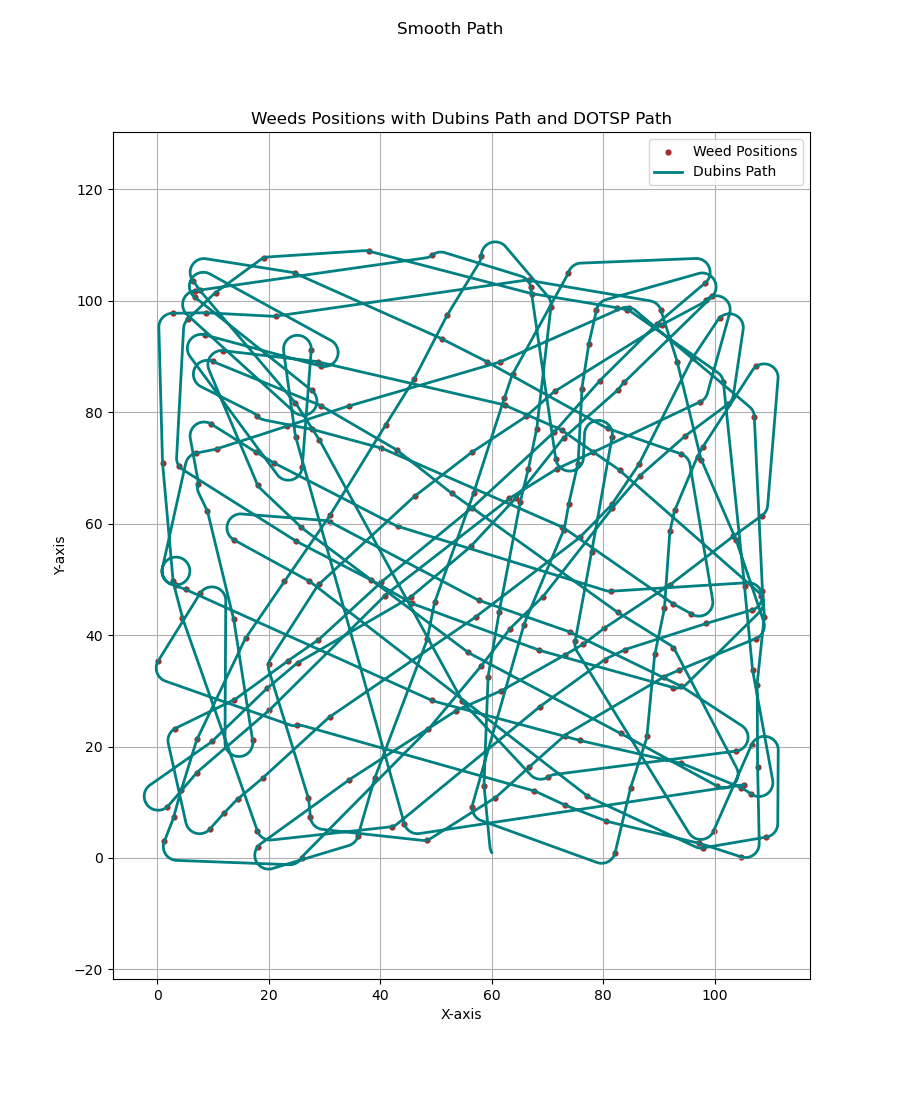
\includegraphics[height=36mm,width=0.24\textwidth]{Images/simulation_no_obs/dubins_path/01.png}
% % % %         & 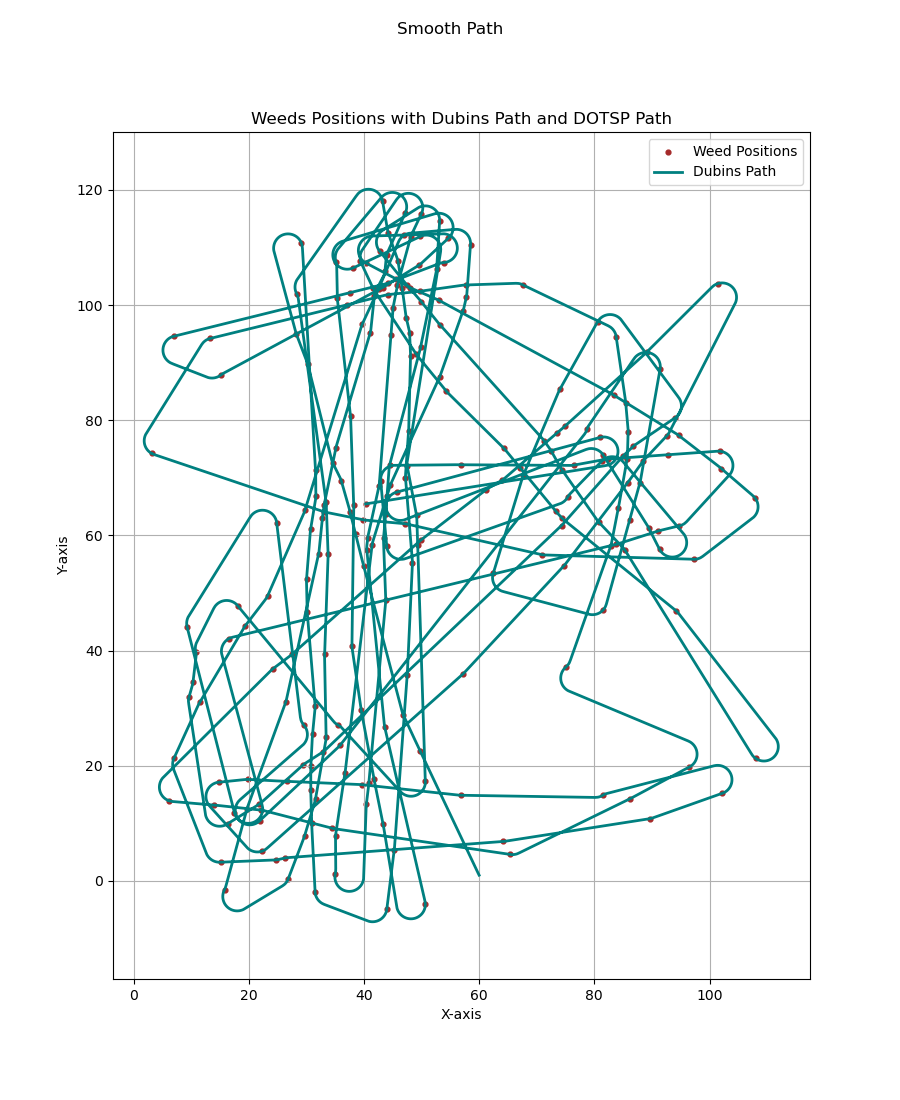
\includegraphics[height=36mm,width=0.24\textwidth]{Images/simulation_no_obs/dubins_path/02.png}
% % % %         & \includegraphics[height=36mm,width=0.24\textwidth]{Images/simulation_no_obs/dubins_path/03.png}
% % % %          \includegraphics[height=36mm,width=0.24\textwidth]{Images/simulation_no_obs/dubins_path/04.png}\\[-4pt]

% % % %         \includegraphics[height=36mm,width=0.24\textwidth]{Images/simulation_no_obs/dubins_path/11.png}
% % % %         & \includegraphics[height=36mm,width=0.24\textwidth]{Images/simulation_no_obs/dubins_path/12.png}
% % % %         & \includegraphics[height=36mm,width=0.24\textwidth]{Images/simulation_no_obs/dubins_path/13.png}
% % % %         \includegraphics[height=36mm,width=0.24\textwidth]{Images/simulation_no_obs/dubins_path/14.png}\\[-4pt]

% % % %         \includegraphics[height=36mm,width=0.24\textwidth]{Images/simulation_no_obs/dubins_path/21.png}
% % % %         & \includegraphics[height=36mm,width=0.24\textwidth]{Images/simulation_no_obs/dubins_path/22.png}
% % % %         & \includegraphics[height=36mm,width=0.24\textwidth]{Images/simulation_no_obs/dubins_path/23.png}
% % % %          \includegraphics[height=36mm,width=0.24\textwidth]{Images/simulation_no_obs/dubins_path/24.png}\\[-4pt]

% % % %          \includegraphics[height=36mm,width=0.24\textwidth]{Images/simulation_no_obs/dubins_path/31.png}
% % % %         & \includegraphics[height=36mm,width=0.24\textwidth]{Images/simulation_no_obs/dubins_path/32.png}
% % % %         & \includegraphics[height=36mm,width=0.24\textwidth]{Images/simulation_no_obs/dubins_path/33.png}
% % % %          \includegraphics[height=36mm,width=0.24\textwidth]{Images/simulation_no_obs/dubins_path/34.png}\\[-4pt]


% % % %         \includegraphics[height=36mm,width=0.24\textwidth]{Images/simulation_no_obs/dubins_path/41.png}
% % % %         & \includegraphics[height=36mm,width=0.24\textwidth]{Images/simulation_no_obs/dubins_path/42.png}
% % % %         & \includegraphics[height=36mm,width=0.24\textwidth]{Images/simulation_no_obs/dubins_path/43.png}
% % % %         \includegraphics[height=36mm,width=0.24\textwidth]{Images/simulation_no_obs/dubins_path/44.png}\\[-4pt]

% % % %         \includegraphics[height=36mm,width=0.24\textwidth]{Images/simulation_no_obs/dubins_path/51.png}
% % % %         & \includegraphics[height=36mm,width=0.24\textwidth]{Images/simulation_no_obs/dubins_path/52.png}
% % % %         & \includegraphics[height=36mm,width=0.24\textwidth]{Images/simulation_no_obs/dubins_path/53.png}
% % % %         \includegraphics[height=36mm,width=0.24\textwidth]{Images/simulation_no_obs/dubins_path/54.png}\\[-4pt]

% % % %     \end{tabular}
% % % %     \caption{Dubin's Path.\label{fig:dubins_path}}
% % % % \end{figure}



\vspace*{6mm}

The performance metrics for all datasets are summarized in the (\autoref{tab:performance_metrics}). These metrics provide insights into the algorithm's computational efficiency, operational effectiveness, and overall robustness.

% % % % % Metrics for CPP.
% % % % \begin{table}[]
% % % %     \centering
% % % %     \caption{Results for the performance metrics.}
% % % %     \label{tab:performance_metrics}
% % % %     \small
% % % %     \begin{tabular}{cllllll}
% % % %     \hline
% % % %     \rowcolor[HTML]{67D5DA} 
% % % %     \multicolumn{1}{l}{\cellcolor[HTML]{67D5DA}\textit{\textbf{\begin{tabular}[c]{@{}l@{}}No. of\\  points\end{tabular}}}} & \textit{\textbf{Cases}} & \textit{\textbf{\begin{tabular}[c]{@{}l@{}}Computation \\ Time in secs.\end{tabular}}} & \textit{\textbf{\begin{tabular}[c]{@{}l@{}}Field Operation\\  Time in sec.\end{tabular}}} & \textit{\textbf{\begin{tabular}[c]{@{}l@{}}Route length\\  in meters\end{tabular}}} & \textit{\textbf{\begin{tabular}[c]{@{}l@{}}No. of \\ Turns.\end{tabular}}} & \textit{\textbf{\begin{tabular}[c]{@{}l@{}}Energy \\ Consumption \\ in KWh.\end{tabular}}} \\ \hline
% % % %     \rowcolor[HTML]{FFFFC7} 
% % % %     \cellcolor[HTML]{FFFFC7}                                                                                               & case 1                  & 0.858553886                                                                            & 6282.400938                                                                               & 4652.945                                                                            & 48                                                                         & 5783.34459                                                                                 \\ \cline{2-7} 
% % % %     \rowcolor[HTML]{FFFFC7} 
% % % %     \cellcolor[HTML]{FFFFC7}                                                                                               & case 2                  & 0.775789261                                                                            & 5125.168209                                                                               & 3769.005                                                                            & 41                                                                         & 4734.555207                                                                                \\ \cline{2-7} 
% % % %     \rowcolor[HTML]{FFFFC7} 
% % % %     \cellcolor[HTML]{FFFFC7}                                                                                               & case 3                  & 0.788151503                                                                            & 5413.822753                                                                               & 3985.978                                                                            & 44                                                                         & 5022.177564                                                                                \\ \cline{2-7} 
% % % %     \rowcolor[HTML]{FFFFC7} 
% % % %     \multirow{-4}{*}{\cellcolor[HTML]{FFFFC7}250}                                                                          & case 4                  & 0.825942278                                                                            & 6216.01818                                                                                & 4620.695                                                                            & 44                                                                         & 5656.894864                                                                                \\ \hline
% % % %     \rowcolor[HTML]{FFFFC7} 
% % % %     \cellcolor[HTML]{FFFFC7}                                                                                               & case 1                  & 1.842700005                                                                            & 9520.140257                                                                               & 7027.363                                                                            & 75                                                                         & 8793.612844                                                                                \\ \cline{2-7} 
% % % %     \rowcolor[HTML]{FFFFC7} 
% % % %     \cellcolor[HTML]{FFFFC7}                                                                                               & case 2                  & 1.696401358                                                                            & 9151.211911                                                                               & 6788.619                                                                            & 67                                                                         & 8366.468569                                                                                \\ \cline{2-7} 
% % % %     \rowcolor[HTML]{FFFFC7} 
% % % %     \cellcolor[HTML]{FFFFC7}                                                                                               & case 3                  & 1.940592766                                                                            & 8589.717644                                                                               & 6336.544                                                                            & 67                                                                         & 7914.394434                                                                                \\ \cline{2-7} 
% % % %     \rowcolor[HTML]{FFFFC7} 
% % % %     \multirow{-4}{*}{\cellcolor[HTML]{FFFFC7}500}                                                                          & case 4                  & 1.609200478                                                                            & 9761.624722                                                                               & 7250.2                                                                              & 70                                                                         & 8898.700417                                                                                \\ \hline
% % % %     \rowcolor[HTML]{FFFFC7} 
% % % %     \cellcolor[HTML]{FFFFC7}                                                                                               & case 1                  & 9.04812026                                                                             & 21751.64778                                                                               & 16189.858                                                                           & 154                                                                        & 19816.55759                                                                                \\ \cline{2-7} 
% % % %     \rowcolor[HTML]{FFFFC7} 
% % % %     \cellcolor[HTML]{FFFFC7}                                                                                               & case 2                  & 8.591621161                                                                            & 22226.37676                                                                               & 16650.701                                                                           & 144                                                                        & 20041.90077                                                                                \\ \cline{2-7} 
% % % %     \rowcolor[HTML]{FFFFC7} 
% % % %     \cellcolor[HTML]{FFFFC7}                                                                                               & case 3                  & 7.65038085                                                                             & 18446.73883                                                                               & 13728.721                                                                           & 131                                                                        & 16813.77138                                                                                \\ \cline{2-7} 
% % % %     \rowcolor[HTML]{FFFFC7} 
% % % %     \multirow{-4}{*}{\cellcolor[HTML]{FFFFC7}2000}                                                                         & case 4                  & 8.155776024                                                                            & 20839.67217                                                                               & 15547.469                                                                           & 139                                                                        & 18820.91894                                                                                \\ \hline
% % % %     \rowcolor[HTML]{FFFFC7} 
% % % %     \cellcolor[HTML]{FFFFC7}                                                                                               & case 1                  & 24.18394971                                                                            & 32301.69933                                                                               & 24191.259                                                                           & 210                                                                        & 29136.75914                                                                                \\ \cline{2-7} 
% % % %     \rowcolor[HTML]{FFFFC7} 
% % % %     \cellcolor[HTML]{FFFFC7}                                                                                               & case 2                  & 20.85941482                                                                            & 29871.08874                                                                               & 22356.011                                                                           & 198                                                                        & 27018.91147                                                                                \\ \cline{2-7} 
% % % %     \rowcolor[HTML]{FFFFC7} 
% % % %     \cellcolor[HTML]{FFFFC7}                                                                                               & case 3                  & 18.23963118                                                                            & 27659.4681                                                                                & 20620.054                                                                           & 192                                                                        & 25141.65448                                                                                \\ \cline{2-7} 
% % % %     \rowcolor[HTML]{FFFFC7} 
% % % %     \multirow{-4}{*}{\cellcolor[HTML]{FFFFC7}4000}                                                                         & case 4                  & 19.22349644                                                                            & 29701.58872                                                                               & 22222.31                                                                            & 200                                                                        & 26932.31049                                                                                \\ \hline
% % % %     \rowcolor[HTML]{FFFFC7} 
% % % %     \cellcolor[HTML]{FFFFC7}                                                                                               & case 1                  & 45.23673987                                                                            & 39851.80224                                                                               & 29777.382                                                                           & 262                                                                        & 35947.48179                                                                                \\ \cline{2-7} 
% % % %     \rowcolor[HTML]{FFFFC7} 
% % % %     \cellcolor[HTML]{FFFFC7}                                                                                               & case 2                  & 33.23154497                                                                            & 34821.16749                                                                               & 26039.854                                                                           & 236                                                                        & 31597.65399                                                                                \\ \cline{2-7} 
% % % %     \rowcolor[HTML]{FFFFC7} 
% % % %     \cellcolor[HTML]{FFFFC7}                                                                                               & case 3                  & 30.80121374                                                                            & 35035.83592                                                                               & 26223.169                                                                           & 230                                                                        & 31639.66906                                                                                \\ \cline{2-7} 
% % % %     \rowcolor[HTML]{FFFFC7} 
% % % %     \multirow{-4}{*}{\cellcolor[HTML]{FFFFC7}6000}                                                                         & case 4                  & 32.34737062                                                                            & 35496.36509                                                                               & 26570.832                                                                           & 226                                                                        & 31893.13207                                                                                \\ \hline
% % % %     \rowcolor[HTML]{FFFFC7} 
% % % %     \cellcolor[HTML]{FFFFC7}                                                                                               & case 1                  & 122.6808474                                                                            & 50681.89334                                                                               & 38128.675                                                                           & 308                                                                        & 45382.07468                                                                                \\ \cline{2-7} 
% % % %     \rowcolor[HTML]{FFFFC7} 
% % % %     \cellcolor[HTML]{FFFFC7}                                                                                               & case 2                  & 74.37674475                                                                            & 45367.87779                                                                               & 34118.252                                                                           & 277                                                                        & 40641.60223                                                                                \\ \cline{2-7} 
% % % %     \rowcolor[HTML]{FFFFC7} 
% % % %     \cellcolor[HTML]{FFFFC7}                                                                                               & case 3                  & 65.54510021                                                                            & 42291.24514                                                                               & 31650.696                                                                           & 278                                                                        & 38197.59611                                                                                \\ \cline{2-7} 
% % % %     \rowcolor[HTML]{FFFFC7} 
% % % %     \multirow{-4}{*}{\cellcolor[HTML]{FFFFC7}10000}                                                                        & case 4                  & 62.76576424                                                                            & 42801.16425                                                                               & 32154.031                                                                           & 274                                                                        & 38606.73138                                                                                \\ \hline
% % % %     \end{tabular}
% % % %     \end{table}



\vspace*{6mm} 


The coverage rate plot over the field time offers a visual representation of the algorithm's performance across the whole datasets. This plot demonstrates how effectively the algorithm achieves coverage over time, allowing for a comparative analysis of its efficiency under varying point distributions and densities. This plot can be visualized in (\autoref{fig:coverage_plots}).   

% % % % % Coverage rate plot
% % % % \begin{figure}[p]
% % % %     \centering
% % % %     \begin{tabular}{ccc}
% % % %          \includegraphics[height=36mm,width=0.24\textwidth]{Images/simulation_no_obs/coverage_plots/01.png}
% % % %         & \includegraphics[height=36mm,width=0.24\textwidth]{Images/simulation_no_obs/coverage_plots/02.png}
% % % %         & \includegraphics[height=36mm,width=0.24\textwidth]{Images/simulation_no_obs/coverage_plots/03.png}
% % % %          \includegraphics[height=36mm,width=0.24\textwidth]{Images/simulation_no_obs/coverage_plots/04.png}\\[-4pt]

% % % %         \includegraphics[height=36mm,width=0.24\textwidth]{Images/simulation_no_obs/coverage_plots/11.png}
% % % %         & \includegraphics[height=36mm,width=0.24\textwidth]{Images/simulation_no_obs/coverage_plots/12.png}
% % % %         & \includegraphics[height=36mm,width=0.24\textwidth]{Images/simulation_no_obs/coverage_plots/13.png}
% % % %         \includegraphics[height=36mm,width=0.24\textwidth]{Images/simulation_no_obs/coverage_plots/14.png}\\[-4pt]

% % % %         \includegraphics[height=36mm,width=0.24\textwidth]{Images/simulation_no_obs/coverage_plots/21.png}
% % % %         & \includegraphics[height=36mm,width=0.24\textwidth]{Images/simulation_no_obs/coverage_plots/22.png}
% % % %         & \includegraphics[height=36mm,width=0.24\textwidth]{Images/simulation_no_obs/coverage_plots/23.png}
% % % %          \includegraphics[height=36mm,width=0.24\textwidth]{Images/simulation_no_obs/coverage_plots/24.png}\\[-4pt]

% % % %          \includegraphics[height=36mm,width=0.24\textwidth]{Images/simulation_no_obs/coverage_plots/31.png}
% % % %         & \includegraphics[height=36mm,width=0.24\textwidth]{Images/simulation_no_obs/coverage_plots/32.png}
% % % %         & \includegraphics[height=36mm,width=0.24\textwidth]{Images/simulation_no_obs/coverage_plots/33.png}
% % % %          \includegraphics[height=36mm,width=0.24\textwidth]{Images/simulation_no_obs/coverage_plots/34.png}\\[-4pt]


% % % %         \includegraphics[height=36mm,width=0.24\textwidth]{Images/simulation_no_obs/coverage_plots/41.png}
% % % %         & \includegraphics[height=36mm,width=0.24\textwidth]{Images/simulation_no_obs/coverage_plots/42.png}
% % % %         & \includegraphics[height=36mm,width=0.24\textwidth]{Images/simulation_no_obs/coverage_plots/43.png}
% % % %         \includegraphics[height=36mm,width=0.24\textwidth]{Images/simulation_no_obs/coverage_plots/44.png}\\[-4pt]

% % % %         \includegraphics[height=36mm,width=0.24\textwidth]{Images/simulation_no_obs/coverage_plots/51.png}
% % % %         & \includegraphics[height=36mm,width=0.24\textwidth]{Images/simulation_no_obs/coverage_plots/52.png}
% % % %         & \includegraphics[height=36mm,width=0.24\textwidth]{Images/simulation_no_obs/coverage_plots/53.png}
% % % %         \includegraphics[height=36mm,width=0.24\textwidth]{Images/simulation_no_obs/coverage_plots/54.png}\\[-4pt]

% % % %     \end{tabular}
% % % %     \caption{Coverage plots.\label{fig:coverage_plots}}
% % % %     \end{figure}


The performance metrics plots provide a visual representation for better understanding of the algorithm's performance across different datasets. Therefore, separate plots for each performance metric are generated to analyze the algorithm's performance under varying scenarios. These plots can be visualized in the (\autoref{fig:Computation_time}), (\autoref{fig:Energy_expenditure}), (\autoref{fig:Route_length}), and (\autoref{fig:Field_operation_time}).


% % % % \begin{figure}[H]
% % % %     \centering
% % % %     \includegraphics[width=\textwidth]{Images/plots/no_obs/Computation_time.png}
% % % %     \caption{Computation Time.}
% % % %     \label{fig:Computation_time}
% % % % \end{figure}

% % % % \begin{figure}[H]
% % % %     \centering
% % % %     \includegraphics[width=\textwidth]{Images/plots/no_obs/Energy.png}
% % % %     \caption{Energy Expenditure.}
% % % %     \label{fig:Energy_expenditure}
% % % % \end{figure}

% % % % \begin{figure}[H]
% % % %     \centering
% % % %     \includegraphics[width=\textwidth]{Images/plots/no_obs/Route_length.png}
% % % %     \caption{Route Length.}
% % % %     \label{fig:Route_length}
% % % % \end{figure}

% % % % \begin{figure}[H]
% % % %     \centering
% % % %     \includegraphics[width=\textwidth]{Images/plots/no_obs/Field_time.png}
% % % %     \caption{Field Operation Time.}
% % % %     \label{fig:Field_operation_time}
% % % % \end{figure}


The proposed algorithm operates by initially generating straight paths and subsequently applying Dubins paths to ensure feasibility given the robot's constraints. The straight paths, as visualized in the initial results, are approximately linear, aiming to cover the maximum number of points while maintaining minimal path length. This demonstrates the algorithm's ability to generate efficient coverage paths.

\vspace*{6mm} 

The Dubins path results further validate the algorithm's capability to model the robot's constraints effectively. An inability to model these constraints accurately would result in numerous infeasible circular paths. The primary objective of employing this behavioral approach is to sustain a high coverage rate from start to finish across various data distributions. The results indicate that the algorithm successfully maintains a high coverage rate irrespective of the distribution type. It is noteworthy that the coverage rate is initially very high and gradually decreases, attributed to the diminishing number of points left to cover after a significant percentage of coverage. Nonetheless, the coverage rate remains high, indicating efficient coverage by the algorithm. The percentage coverage also suggests that the point at which the algorithm changes behavior is near-optimal; otherwise, a gradual increase in coverage rate would be observed if the change occurred at a different percentage.

\vspace*{6mm} 

The computation time plot across all datasets indicates an expected increase in computation time with the number of points. However, the rise in computation time is notable. For instance, even in the largest case of 10,000 points with random distribution, the computation time is 122.68 seconds, which is remarkably low as compared to current state-of-the-art approaches following the non-holonoomic constraints. This efficiency is further highlighted by the average computation time of 60 seconds for other scenarios, demonstrating the algorithm's computational efficiency. This is particularly significant as no real agricultural field would have a purely random distribution, making the algorithm's performance even more impressive in practical scenarios.

\vspace*{6mm} 

Similarly, the route length increases with the number of points as the robot needs to traverse more straight lines to cover all points. It is noteworthy that the maximum route length for each dataset occurs with random distribution and decreases significantly with fewer clusters, increasing again as the number of clusters rises.

\vspace*{6mm} 

Field operation time and energy consumption are derived from the route length, factoring in the robot's maximum allowable velocity on straight and curved paths. The robot can move at twice the speed on straight paths compared to curved paths without damaging crops. The parameters used for the current robot, as outlined in the table, provide a close approximation of real values, although the exact curved distance is challenging to estimate with this pipeline. Energy consumption is approximated to be four times higher on curved paths than on straight paths. The plots above reflect these estimations. 














